%%%%%%%%%%%%%%%%%%%%%%%%%%%%%%%%%%%%%%%%%%%%%%%%%%%%%%%%%%%%%%%%%%%%%%%%%%%% 
% AGUJournalTemplate.tex: this template file is for articles formatted with LaTeX
% 
% This file includes commands and instructions
% given in the order necessary to produce a final output that will
% satisfy AGU requirements, including customized APA reference formatting.
% 
% You may copy this file and give it your
% article name, and enter your text.
% 
% 
% Step 1: Set the \documentclass
% 
% 

%% To submit your paper:
\documentclass[draft]{agujournal2019}
\usepackage{url} %this package should fix any errors with URLs in refs.
\usepackage{lineno}
\usepackage{hyphenat}
\usepackage{float}
\usepackage{multirow}
\usepackage[inline]{trackchanges} %for better track changes. finalnew option will compile document with changes incorporated.
\usepackage{soul}
\usepackage{array}
\newcolumntype{L}[1]{>{\raggedright\arraybackslash}p{#1}}
\newcolumntype{C}[1]{>{\centering\arraybackslash\hspace{0pt}}p{#1}}

\linenumbers
\sloppy
\hbadness=99999 
%%%%%%% 
% As of 2018 we recommend use of the TrackChanges package to mark revisions.
% The trackchanges package adds five new LaTeX commands:
% 
% \note[editor]{The note}
% \annote[editor]{Text to annotate}{The note}
% \add[editor]{Text to add}
% \remove[editor]{Text to remove}
% \change[editor]{Text to remove}{Text to add}
% 
% complete documentation is here: http://trackchanges.sourceforge.net/
%%%%%%% 

\draftfalse

%% Enter journal name below.
%% Choose from this list of Journals:
% 
% JGR: Atmospheres
% JGR: Biogeosciences
% JGR: Earth Surface
% JGR: Oceans
% JGR: Planets
% JGR: Solid Earth
% JGR: Space Physics
% Global Biogeochemical Cycles
% Geophysical Research Letters
% Paleoceanography and Paleoclimatology
% Radio Science
% Reviews of Geophysics
% Tectonics
% Space Weather
% Water Resources Research
% Geochemistry, Geophysics, Geosystems
% Journal of Advances in Modeling Earth Systems (JAMES)
% Earth's Future
% Earth and Space Science
% Geohealth
% 
% ie, \journalname{Water Resources Research}

\journalname{Geophysical Research Letters}

\newcommand{\aref}[1]{\textbf{Reference #1}}
\newcommand{\TODO}[1]{\textbf{TODO #1}}
\newcommand{\ian}[1]{{\textbf{\color{blue}Ian says:} \color{blue} #1} }
\newcommand{\leif}[1]{{\textbf{\color{red}Leif says:} \color{red} #1} }
\newcommand{\db}{\textit{DEBRIS}\,}
\newcommand{\cl}{\textit{CLEAN}\,}
\newcommand{\m}{$\,\mathrm{m}$\,}
\newcommand{\cm}{$\,\mathrm{cm}$\,}
\newcommand{\mma}{$\,\mathrm{mm  \, a^{-1}}$\,}
\newcommand{\mmma}{$\,\mathrm{m^3\, a^{-1}}$\,}
\newcommand{\mmms}{$\,\mathrm{m^3\, s^{-1}}$\,}
\newcommand{\unit}[1]{$\mathrm{#1}$}


\newenvironment{laysummary}{
  \chapter{\centering \textbf{Plain Language Summary}}
}



\begin{document}
%% ------------------------------------------------------------------------ %%
% Title
% 
% (A title should be specific, informative, and brief. Use
% abbreviations only if they are defined in the abstract. Titles that
% start with general keywords then specific terms are optimized in
% searches)
% 
%% ------------------------------------------------------------------------ %%

% Example: \title{This is a test title}


\title{Comparing variations in sediment transport capacity between subglacial and subaerial channels } 


%% ------------------------------------------------------------------------ %%
% 
% AUTHORS AND AFFILIATIONS
% 

% Authors are individuals who have significantly contributed to the
% research and preparation of the article. Group authors are allowed, if
% each author in the group is separately identified in an appendix.)

% List authors by first name or initial followed by last name and
% separated by commas. Use \affil{} to number affiliations, and
% \thanks{} for author notes.
% Additional author notes should be indicated with \thanks{} (for
% example, for current addresses).

% Example: \authors{A. B. Author\affil{1}\thanks{Current address, Antarctica}, B. C. Author\affil{2,3}, and D. E.
% Author\affil{3,4}\thanks{Also funded by Monsanto.}}

\authors{Ian Delaney\affil{1}}


\affiliation{1}{Institut des dynamiques de la surface terrestre (IDYST), Universit\'{e} de Lausanne, B\^{a}timent G\'{e}opolis, CH-1015 Lausanne }

% \affiliation{3}{Third Affiliation}
% \affiliation{4}{Fourth Affiliation}

% \affiliation{=number=}{=Affiliation Address=}
% (repeat as many times as is necessary)

%% Corresponding Author:
% Corresponding author mailing address and e-mail address:

% (include name and email addresses of the corresponding author.  More
% than one corresponding author is allowed in this LaTeX file and for
% publication; but only one corresponding author is allowed in our
% editorial system.)

% Example: \correspondingauthor{First and Last Name}{email@address.edu}

\correspondingauthor{Ian Delaney}{ianarburua.delaney@unil.ch}



%% Keypoints, final entry on title page.

% List up to three key points (at least one is required)
% Key Points summarize the main points and conclusions of the article
% Each must be 140 characters or fewer with no special characters or punctuation and must be complete sentences

% Example:
% \begin{keypoints}
% \item	List up to three key points (at least one is required)
% \item	Key Points summarize the main points and conclusions of the article
% \item	Each must be 140 characters or fewer with no special characters or punctuation and must be complete sentences
% \end{keypoints}



\begin{keypoints}
\item Water discharge variations in subglacial channels are accommodated by water velocity, not channel size, given their slow evolution.

\item Greater variability in water velocity in subglacial systems causes sediment transport capacity to vary more than subaerial systems.


\item The systems' divergence in transport response may impact sediment dynamics at glacier margins and interpretation of sediment records.
\end{keypoints}


%% ------------------------------------------------------------------------ %%
% 
% ABSTRACT and PLAIN LANGUAGE SUMMARY
% 
% A good Abstract will begin with a short description of the problem
% being addressed, briefly describe the new data or analyses, then
% briefly states the main conclusion(s) and how they are supported and\cite <e.g.,>[and others]{lewin76}
% uncertainties.

% The Plain Language Summary should be written for a broad audience,
% including journalists and the science-interested public, that will not have 
% a background in your field.
% 
% A Plain Language Summary is required in GRL, JGR: Planets, JGR: Biogeosciences,
% JGR: Oceans, G-Cubed, Reviews of Geophysics, and JAMES.
% see http://sharingscience.agu.org/creating-plain-language-summary/)
% 
%% ------------------------------------------------------------------------ %%

%% \begin{abstract} starts the second page 

\begin{abstract} % 150 words
Sediment transport capacity depends mainly on the shear stress or velocity of water flowing through a channel and the channel width over which to mobilize sediment.
In subaerial channels, changing water discharge can be accommodated by rapid changes in the channel width over which water flows, the water depth, and the water velocity.
In subglacial channels, however, water flows through a conduit whose size evolves  slowly, because the water is pressurized by the glacier ice above.
As a result, variations in water discharge may modify the water velocity, but not the channel's width.
Here, parameterizations of subglacial and subaerial channels indicate that sediment transport capacity varies more in subglacial systems compared with subaerial systems, across a wide range of channel geometries and flow conditions.
Large variations in subglacial water sediment transport capacity may impact sediment transport processes and the interpretation of records of sediment transport from glacierized catchments.

  
\end{abstract}

\section*{Plain language summary} % 200 words
In both subglacial and subaerial channels, sediment transport capacity depends mainly on 1) the channel width over which the sediment is mobilized  and 2) the shear stress applied by flowing water on sediment at the channel bottom; the shear stress depends mainly on the water velocity.
In subaerial channels, changing water discharge will  change the water depth,  the channel width (which dictates the distance  over which sediment transport  occurs), and the  water velocity (which controls the sediment transport capacity).
 In subglacial environments, however, on times scales of hours to weeks, changing water discharge will only alter  water velocity, not channel area, because the subglacial conduit maintains a largely fixed geometry.
The fixed conduit geometry also means that the channel width over which the sediment is  mobilized also does not respond to changing water discharge.
Parameterizations of these processes show that sediment transport capacity varies far more in subglacial systems compared to subaerial systems, even though changing channel width can accommodate some sediment transport variability in subaerial channels.
The increased variability in sediment transport capacity in subglacial systems, compared to subaerial ones, has several important implications for sediment transport in glacierized catchments and the interpretation of sediment discharge records.


%% ------------------------------------------------------------------------ %%
% 
% TEXT
% 
%% ------------------------------------------------------------------------ %%

%%% Suggested section heads:
\section{Introduction}
\label{sect:intro}


  Glaciers expel large quantities of sediment from their termini \cite{hallet1996}.
  Changes in glacier dynamics, geomorphology, and hydrology  have prompted numerous  recent studies of  sediment transport processes in cold regions \cite<e.g.>[]{zhang2022}.
  Increases in sediment transport  have been observed in Greenland \cite{bendixen2017}, the European Alps \cite{costa2017}, the Himalayas \cite{li2021}, and the Andes \cite{vergara2022}.
  In some of these regions, increased water discharge and glacier melt have been attributed to greater sediment transport \cite{bendixen2017,costa2017,li2021}.
  In other cases, enhanced access of meltwater to subglacial sediment at high elevations was attributed as the cause of increased sediment transport \cite{delaney2020,vergara2022}.
  Observed changes to sediment transport in glacierized catchments create an imperative to examine the processes controlling sediment discharge here. 
  Yet, the relationship between water discharge and sediment transport in subglacial environments remains minimally discussed and not contrasted with the subaerial river systems that these glaciers feed.
 
  Over long periods, processes such as glacier abrasion and quarrying sculpt landscapes and create sediment to be transported fluvially from below glaciers \cite<c.f.>{hallet1979,iverson2012,ugelvig2018}. 
  On shorter time periods, pressurized water transports sediment from the below glacier \cite{walder1994,creyts2013,beaud2018}, should enough sediment be present below the glacier (i.e. in a transport-limited regime).
  
  In a transport-limited regime, sediment discharge responds to the sediment transport capacity or the amount of sediment that could be carried by the water. Sediment transport capacity depends on the shear stress between water and sediment it flows  over \cite{shields1936,meyer1948,engelund1967} and the width of the channel bottom $w_c$ over which to mobilize sediment. The shear stress  across the channel width $\tau_t$ responds to the velocity of water $v$ flowing through at channel so that 
  \begin{linenomath*}
    \begin{equation}
      \label{eq:tau_t}
      \tau_t \propto w_c\, v^2,
    \end{equation}
  \end{linenomath*}
  % 
  where $w_c$ is the width of the channel.
  Following the conservation of mass, the velocity of the water flowing through a rectangular channel is given as 
  \begin{linenomath*}
    \begin{equation}
      \label{eq:v}
      v = \frac{Q_w}{S},
    \end{equation}
  \end{linenomath*}
  % 
  where $Q_w$ is water discharge,  and $S$ is the channel's cross-sectional area.

  In subaerial channels, with open channel flow, the cross-sectional area $S$ of the channel evolves with changing water discharge $Q_w$  by changing the width of the channel along with the depth \cite{leopold1953}. During a flood with greater water discharge $Q_w$, for instance, the cross-sectional area $S$ increases as the channel widens and deepens, along with water velocity $v$. As a result, the shear stress across the channel $\tau_t$ will increase in response to both the channel width $w_c$  and water velocity $v$. 

  Yet, the response of water velocity to changing water discharge in subglacial channels is different than subaerial ones.
  In subglacial systems, the water is pressurized by the ice above \cite{shreve1972}.
  The size of subglacial channels responds to the creep closure of the ice above and the opening of the channel by frictional heating of water flowing through the channel \cite{rothlisberger1972}.
  As a result, the subglacial channel size evolves over days to months, whereas water discharge varies over hours \cite<e.g.>[]{iken1986,andrews2014,nanni2020}.
  In turn, changes in water discharge $Q_w$ are mainly accommodated with water velocity $v$, because the size of the channel $S$ is largely fixed (Equation~\ref{eq:v} and Figure~\ref{fig:cartoon}).
  It follows that greater water discharge $Q_w$ will cause the shear stress across the channel $\tau_t$ to respond to the water velocity $v$, as opposed to the subaerial system where width evolves as well. 

  As a result, sediment mobilization in subaerial and subglacial systems responds differently to changing water discharge.
  These differences have been implicitly included in a wide range of available models that  quantify sediment transport from catchments in both subglacial and subaerial systems  \cite<e.g.>[]{walder1994,tucker1997,creyts2013,wickert2019,hewitt2019}.
  The divergent response of changing water discharge on sediment mobilization capacity may well impact sediment dynamics at glacier margins where flow transitions from pressurized to open channel flow \cite<e.g.>[]{lane2016}.
  Additionally, the variable response of sediment transport capacity to water discharge in the two systems may impact the interpretation of records of sediment transport in glacial compared to subaerial systems \cite<e.g.>[]{muller1968,richards2003,ganti2016}.
  Yet, the differing relationship between variations in water discharge and sediment discharge in subglacial and subaerial systems has been minimally discussed.
  
  This manuscript leverages parameterizations of subglacial and subaerial hydraulics to explore differences in the relationships between  water discharge, channel geometry, and water velocity. 
  With these parameterizations, the manuscript examines the impact of water discharge variability on sediment transport capacity in idealized subglacial and subaerial systems.
  Lastly, the manuscript discusses the implications for sediment transport processes in subglacial systems, compared to subaerial ones.
  
  \begin{center}
    \begin{figure}[H]
      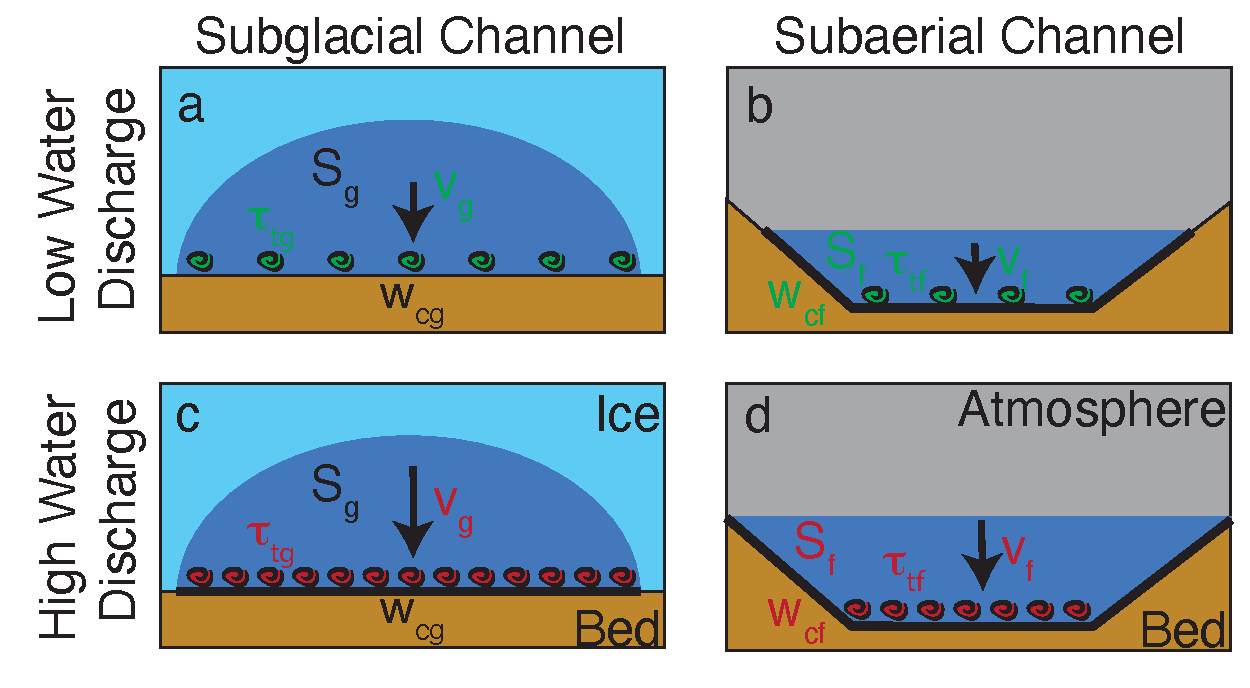
\includegraphics[width=0.8\linewidth]{Fig1.pdf}
      \caption{Cartoon of the situation with various parameters. Water velocity magnitude in the subglacial, $v_g$, and subaerial, $v_f$, systems are shown by arrow length. $S_g$ and $S_f$ represent the cross-sectional area in subglacial and subaerial channels. The subglacial channel widths $w_{cg}$ remain steady, while the subaerial channel widths evolve $w_{cf}$, denoted by the thick black line. Shear stress $\tau$ is responsible for the mobilization of sediment and increases with the number of makers at the channel bed. 
        Note that in the subaerial channel parameterization, rectangular channel shapes are implemented (Section~\ref{sect:fluv}).} 
      \label{fig:cartoon}
    \end{figure}
  \end{center}


\section{Methods}
\label{sect:meth}
    Parameterizations below represent relationships amongst water discharge, subglacial water velocity, and channel geometry in both subaerial and subglacial channels (Table \ref{table:vpm}).
  Because sediment transport largely depends on shear stress applied by water flow \cite{shields1936}, both parameterizations calculate this value and integrate  it across the channel bed (Figure \ref{fig:cartoon}).
  The evaluation of shear stress omits a grain size parameter and, thus, leaves open the selection of a sediment transport relationship  \cite<e.g.>[]{shields1936,meyer1948} to  calculate sediment transport capacity.
  As a result, relative relationships in shear stress, as opposed to sediment transport capacity, are examined.

  \begin{table}[H]
    \centering
    \caption{Variables, parameters, and constants }
    \begin{tabular}{ l  c  c c }
      Name &Symbol&  Value&Units \\ \hline
      \textbf{Variables}  & & & \\
      Channel hydraulic diameter (glacier, subaerial) &  $D_{hg},\,D_{hf}$&  & $\mathrm{m}$     \\
      Width of channel floor (glacial, subaerial) & $w_{cg},w_{cf}$&  & $\mathrm{m}$     \\
      Channel cross-sectional area (glacier, subaerial) &  $S_g, S_f$& & $\mathrm{m^2}$     \\
      Water discharge (instantaneous) & $Q_w$& & $\mathrm{m^{3}\,s^{-1}}$ \\
      Representative water discharge & $Q_{w}^*$& & $\mathrm{m^{3}\,s^{-1}}$ \\
      Representative hydraulic gradient  &$\Psi^*$ & & $\mathrm{Pa\, m^{-1}}$\\
      Water velocity (glacier, subaerial)  & $v_g,\,v_{f}$& & $\mathrm{m\,s^{-1}}$ \\
      Shear stress (glacier, subaerial) & $\tau_g,\,\tau_f$&& $\mathrm{Pa \, m^{-1}}$ \\
      Width-integrated shear-stress (glacier, subaerial) & $\tau_{tg},\, \tau_{tf}$&& $\mathrm{Pa \, m^{-1}}$ \\
      Reynolds number &$R_e$& & $\mathrm{(-)}$\\
      Variable &$\Gamma$&&$\mathrm{(-)}$\\
      Variability of a variable ($\Gamma$) &$\chi$& &$\mathrm{(-)}$\\
           &&&\\
      
      \textbf{Parameters and Constants}  & & &\\
      Gravitational constant&$g$& $-9.81$&$\mathrm{m\,s^{-2}}$\\
      Density of water & $\rho_w$& $1000$ & $\mathrm{kg\,m^{-3}}$ \\
      Density of ice & $\rho_i$& $900$ & $\mathrm{kg\,m^{-3}}$ \\
      Kinematic viscosity of water &$\nu$& $10^{-4}$& $\mathrm{m^2\,s^{-1}}$\\
      Hooke angle of channel & $\beta$ & $\frac{\pi}{2}$ & \unit{rad}\\
      Flotation fraction & $f_f$&$0.7$& $\mathrm{(-)}$\\
      Friction factor (glacier) & $f_r$ & $4$ & $\mathrm{(-)}$ \\
      Friction factor (subaerial) & $f_p$ & $3$ & $\mathrm{(-)}$\\
      Gradient of glacier surface & $\frac{\partial z_{sg}}{\partial x}$ &$0.25$& $\mathrm{(-)}$\\
      Gradient of channel bed (subaerial) &$\frac{\partial z_c}{\partial x}$ &$0.05$& $\mathrm{(-)}$\\
      Subaerial channel factor & $k$ &$3$ & $\mathrm{s\,m^{-2}}$\\
      Channel geometry exponent &$e$& $\frac{1}{2}$&$\mathrm{(-)}$ \\
      \hline
    \end{tabular}
    \label{table:vpm}
  \end{table}
  
  \subsection{Subglacial channel  parameterization}
  \label{sect:sub_mode}
  To evaluate the shear stress of water flowing across sediments below a glacier, the subglacial channel parameterization evaluates the channel geometry and the velocity of the flowing water.
  To accomplish this, the hydraulics model presented in \citeA{delaney2019} is used.
  
  Here, it is assumed that the water is transported through subglacial channels \cite<Figure~\ref{fig:cartoon}; >{rothlisberger1972}, and that the channel  geometry will respond to a representative water discharge over a certain time period $Q_{w}^*$, using the Darcy-Weisbach formulation for water-flow through a pipe  \cite<e.g.>[]{rothlisberger1972,clarke2003,werder2013}.
  Thus, the hydraulic diameter of the subglacial channel, $D_h$, responds to a representative water discharge, $Q_{w}^*$, and a representative gradient of the hydraulic potential, $\Psi^*$ such that:
  \begin{linenomath*}
    \begin{equation}
      \label{eq:DW}
      D_h = \big(s\, f_r\,\rho_w\, \frac{Q_w^{*\,2}}{\Psi^*}\big)^{\frac{1}{5}}~~.
    \end{equation}
  \end{linenomath*}
  % 
  The representative hydraulic gradient is based upon the pressurized flow in Equation~\ref{eq:DW},
  \begin{equation}
    \label{eq:psi}
    \Psi^*= f_f \,  \rho_i \, g (\frac{\partial  z_{sg}}{\partial x} - \frac{\partial z_c}{\partial x}) +  \rho_i \, g \, \frac{\partial z_c}{\partial x},
  \end{equation}
  % 
  \noindent
  where, $f_f$ is the flotation fraction, $\rho_i$ is density of ice $\frac{\partial z_{sg}}{\partial x}$ is the surface slope of the glacier and $\frac{\partial z_c}{\partial x}$ is the glacier bed slope.
  
  In Equation~\ref{eq:DW}, $f_r$ is the Darcy-Weisbach friction factor and $\rho_w$ is the density of water (Table \ref{table:vpm}). $s$ is a factor accounting for channel geometry \cite{hooke1990}, calculated as:
  \begin{equation}
    \label{eq:Hf}
    s = \frac{2\,(\beta -\sin \beta)^2}{(\frac{\beta}{2}\,+\,\sin \frac{\beta}{2})^4},
  \end{equation}
  where $\beta$ is the central angle of the circular segment that comprises the channel (the so-called Hooke angle). Note that $\beta =\pi$ corresponds to a semi-circle and
  smaller values of $\beta$ result in shallow, wide channels. 
  The width of the flat channel floor $w_c$, given angle $beta$ is 
  \begin{equation}
    \label{eq:dh2wc}
    w_{cg} = 2  \sin \frac{\beta}{2} \sqrt{\frac{2\, S}{\beta -\sin \beta}},
  \end{equation}
  % 
  where $S$ is the cross-sectional area of the channel given by
  \begin{equation}
    \label{eq:dh2S}
    S_g =  \frac{D_h^2}{2}~ \frac{\Big(\frac{\beta}{2} \,+ \, \sin \frac{\beta}{2}\Big)^2  }{\beta\,-\,\sin \beta}.
  \end{equation}
  
  The shear stress, $\tau$, between the water and the channel bed is determined through the Darcy-Weisbach formulation
  \begin{equation}
    \label{eq:tau}
    \tau_g=\frac{1}{8}\,f_r\,\rho_w\,v_g^2,
  \end{equation}
  % 
  where  the water velocity $v_g$ is $v_g = \frac{Q_w}{S_g}$.
  Here, $Q_w$ represents the instantaneous water discharge, rather than $Q_w^*$, which is used to evaluate the channel geometry.
  With this formulation, the processes in an R-channel, through which water flows subglacially, can be represented algebraically \cite{rothlisberger1972,delaney2019}.
  
    Width integrated shear stress is represented as $\tau_{tg}=w_{cg}\,\tau_g $.
  
  \subsection{Subaerial channel  parameterization}
  \label{sect:fluv}
  
  To parameterize the shear stress of water flowing across sediments in the subaerial channel,  the hydraulics parameterization presented in \citeA{tucker1997} is implemented.
  Here, it is assumed that there is a conservation of mass and a sufficiently wide channel so that the hydraulic radius is consistent with flow depth, uniform flow, and the Darcy-Weisbach relationship.
  The shear stress $\tau_f$ at the river bed is represented as
  \begin{linenomath*}
    \begin{equation}
      \label{eq:DW_tau}
      \tau_f=\frac{\rho_w\,g^{\frac{2}{3}}\,f_p^{\frac{1}{3}}}{2}\, \Big(\frac{Q_w}{w_{cf}} \Big)^{\frac{2}{3}} \,\frac{\partial z_c}{\partial x}^{\frac{2}{3}},
    \end{equation}
  \end{linenomath*}
  where $\frac{\partial z_c}{\partial x}$ is the channel slope, and $f_p$ is the friction factor for subaerial systems.
  Channel width $w_{cf}$ is 
  \begin{equation}
    \label{eq:wcf}
    w_{cf} = k \, Q_w^e,
  \end{equation}
  % 
  where $k$ is a constant and $e$ is an exponent commonly equal to $\frac{1}{2}$ \cite{leopold1953}.
  Cross-sectional area, $ S_f$, is 
  \begin{equation}
    \label{eq:Sf}
    S_f = \frac{Q_w}{v_f},
  \end{equation}
  % 
  where $v_f$ is water velocity, given by rearranging Equation \ref{eq:tau} as
  \begin{equation}
    \label{eq:vf}
    v_f = \sqrt{\frac{8\,\tau_f}{f_p\,\rho_w}}.
  \end{equation}
  % 
  As in Section~\ref{sect:sub_mode}, the width integrated shear stress is $\tau_{tf}=w_{cf}\,\tau_f$.
  Hydraulic diameter of the channel is given by $D_{hf} = \frac{4\,w_{cf}\,d}{2\,d+w_{cf}}$, with flow depth $d$ determined from knowledge of $S_f$ and $w_{cf}$ in a rectangular channel.
  
  \subsection{Implementation}
  
  The formulation of the glacial system (Section~\ref{sect:sub_mode}) requires inputs of the hydraulic gradient (Equation \ref{eq:psi}; $\frac{\partial z_{sg}}{\partial x}$, $\frac{\partial z_{c}}{\partial x}$), water discharge, $Q_w$ representative water discharge, $Q_w^*$,  Hooke angle (Equation~\ref{eq:Hf}; $\beta$), and friction factor (Equation~\ref{eq:DW}; $f_r$).

  
  In the subaerial system,  only the bed slope, $\frac{\partial z_c}{\partial x}$, is needed in Equation~\ref{eq:DW_tau}. The friction factor, $f_f$, and channel shape factor, $k$, are assigned such that they produce reasonable values for water velocity and channel width  (Section~\ref{sect:fluv}).
  
  The Reynolds number $R_e$, which gives an evaluation of the degree of turbulence of the water, is given as 
  \begin{equation}
    \label{eq:re}
    R_e\,=\, v \,\frac{D_h}{\nu},
  \end{equation}
  % 
  \noindent where $\nu$ is the kinematic viscosity of water, and  $v$ is velocity of water, $v_g$ or $v_f$.
  
  The variance $ \chi$ of a variable $\Gamma$ is given by 
  \begin{equation}
    \label{eq:var}
    \chi(\Gamma) \,=\, 1 - \frac{\mathrm{min}(\Gamma)}{\mathrm{max}(\Gamma)}\,\,.
  \end{equation}
  % 
  \noindent Below we examine variables, $\Gamma$, as water discharge ($Q_w$) water velocity ($v_g$, $v_f$), shear stress ($\tau_g$, $\tau_f$), and integrated shear stress ($\tau_{tg}$, $\tau_{tf}$) with the purpose of evaluating total shear stress across the glacier bed.

\section{Results}
  Initially, both parameterizations are forced with a water discharge ($Q_w$) varying between $8$ and $16$ \,\unit{m}$^{3}$\,\unit{s}$^{-1}$, to represent a range of sediment transport conditions, for instance over diurnal fluctuation in water discharge. The subaerial channel width factor $k$ is $3$\,\unit{m}$^{2}$\,\unit{s}$^{-1}$, and the Hooke angle $\beta$ is $\frac{\pi}{2}$.
  Values of Hooke angle $\beta$ and subglacial friction factor $f_r$ are chosen so that they produce reasonable values of water velocity ($0.6- 1.2$\,\unit{m}\,\unit{s}$^{-1}$) in accordance with measurements made through dye-tracing experiments to examine subglacial hydraulic conditions \cite<Section~\ref{sect:sub_mode}, Figure~\ref{fig:model_outs}; e.g.>{werder2010}.
  The subglacial representative water discharge ($Q_w^*$; Equation~\ref{eq:DW}) of $12$\,\unit{m}$^{3}$\,\unit{s}$^{-1}$ is applied to establish the hydraulic diameter and shape of the channel.
  
  \begin{center}
    \begin{figure}[H]
      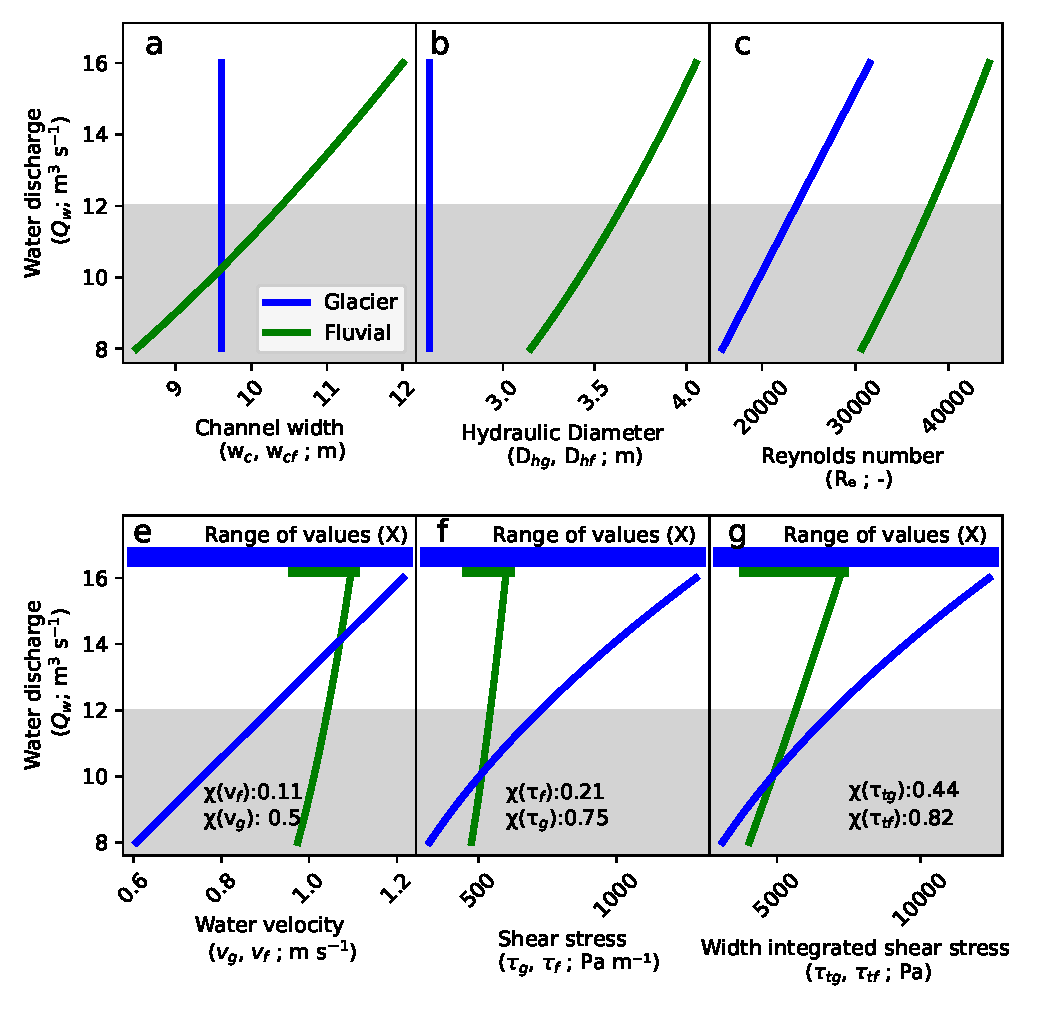
\includegraphics[width=0.8\linewidth]{model_outputs.pdf}
      \caption{Response of channel width (a), hydraulic diameter (b),  Reynolds number  (c),  water velocity (d), shear-stress (e), and width-integrated shear-stress (f)  to different water discharge values. The glacial system is in blue and the subaerial system is in green.  Horizontal bars in d, e, and f represent the range of values in the  output. Gray space represents water discharge below the mean value. }
      \label{fig:model_outs}
    \end{figure}
  \end{center}
  
  Across the hydrological forcing, variable water discharge results in a substantial increase in the range of water velocities in the glacial system compared to the subaerial system (Figure~\ref{fig:model_outs}).
  Water velocity in the glacier system varies by  $0.5$ (Equation~\ref{eq:var}) over the discharge values, in the subaerial system the water velocity only varies by $0.11$ (Figure~\ref{fig:model_outs}\,e).
  Shear stress at the glacier bed varies by $0.75$ across the range of water discharge values, whereas shear stress across the subaerial system varies by roughly $0.21$ (Figure~\ref{fig:model_outs}\,f). The increased variability in shear stress relative to water velocity between the two systems occurs as the water velocity is raised to the power of $2$ in Equation~\ref{eq:tau}. 
  
  In the subaerial systems, changing channel geometry accommodates evolving water discharge  (Equation~\ref{eq:wcf}), whereas in the subglacial case, increased water flux can only result in changing water velocity (Equations~\ref{eq:v}~ and ~\ref{eq:DW}).
  As a result, in the subaerial system, variability in the shear stress $\tau_f$ and width-integrated shear stress $\tau_{tf}$ increases from $0.21$ to $0.44$. Variability in width-integrated shear stress  in the glacial system $\tau_{tg}$ is $0.83$ (Figure~\ref{fig:range}).
  The reduced variability in width-integrated shear stress results from the additional width across the subaerial channel that accommodates some variations in water discharge.
  Indeed, the relative  difference in width-integrated shear stress is less between the subaerial and glacier cases, compared to the water velocity and shear stress outputs (Figure~\ref{fig:model_outs}\,e--g).

  
  Next, the parameterizations are run $25,000$ times with randomly selected channel geometries ($k=(2,6)$, $\beta=(\frac{\pi}{10},\pi)$), friction factors ($f_i=(0.001,20)$, $f_p=(0.001,20)$) and water discharges (maximum and minimum values selected between $5$ to $500$ \,\mmms). $Q_w^*$ in Equation ~\ref{eq:DW} is determined from the mean in the water discharge range. Parameter combinations are only selected if their maximum and minimum velocities for both the subglacial and subaerial systems are between $0.2$ and $3$\,\unit{m}\,\unit{s}$^{-1}$, resulting in roughly $10,600$ adequate parameter combinations. 
  
  
  \begin{center}
    \begin{figure}[H]
      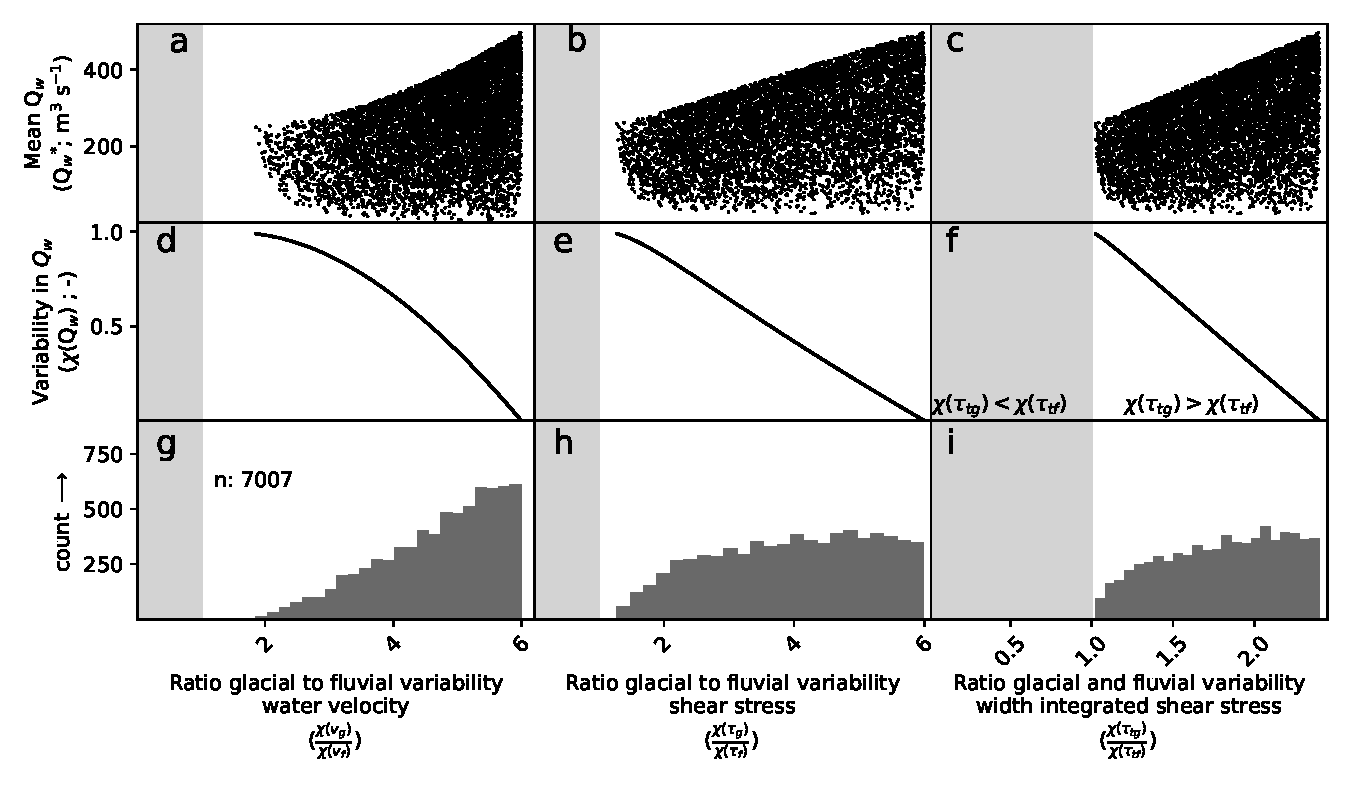
\includegraphics[width=0.8\linewidth]{multi_run.pdf}
      \caption{Ratio of range of water velocity, shear-stress, and width integrated shear-stress for glacial and subaerial systems in response to mean water discharge (a, b, c), and  variability in water discharge (d, e, f).  
        Range  $\chi$ for each variable is given in Equation~\ref{eq:var}. Values greater than $1$ shown in white space are parameter combinations that vary more in a subglacial  system.
        Histograms (g-i) show the frequency of relative variations across variables in the parameterization.}
      \label{fig:range}
    \end{figure}
  \end{center}
  
  Across the accepted model runs, variability in water velocity and shear stress remains substantially higher across the subglacial model compared to subaerial ones (Figure~\ref{fig:range}).
  Water velocity, shear stress, and width-integrated shear stress all have a variability ratio ($\frac{\chi(\Gamma_{g})}{\chi(\Gamma_f)}$) greater than $1$ in the subglacial  system compared to subaerial one (Figure~S \ref{fig:gammas}).
  Runs with the smallest variability in discharge ($\chi(Q_w)$) have the greatest variability in water velocity, shear stress, and width-integrated shear stress in subglacial systems compared to subaerial ones (Figure~\ref{fig:range}\,d--f and S \ref{fig:gammas}).
  
  The minimum ratio of  water velocity, $\frac{\chi(v_{g})}{\chi(v_{f})}$, and shear-stress, $\frac{\chi(\tau_{g})}{\chi(\tau_{f})}$, is greater than $1.5$.
  These results show that increased variability occurs across a wide range of subaerial and subglacial channel configurations (Figure~\ref{fig:range} g, h).
The width integrated shear stress, $\frac{\chi(\tau_{tg})}{\chi( \tau_{tf})}$, spans between $1.02$ and $2.4$, a smaller amount of relative variability compared to  water velocity $\frac{\chi(v_{g})}{\chi(v_{f})}$ or shear stress $\frac{\chi(\tau_{g})}{\chi(\tau_{f})}$ (Figure~\ref{fig:range}).
Consistent with the individual case (Figure ~\ref{fig:model_outs}), the subaerial systems' reduce variability in width-integrated shear stress occurs  as the evolving channel width accommodates some of the reduced shear stress variability in subaerial systems (Figure~\ref{fig:range} i).
  Importantly though, no runs experienced relative variability in width integrated shear stress, $\frac{\chi(\tau_{tg})}{\chi( \tau_{tf})}$, less than $1$, showing that the subglacial has consistently high variability in width integrated shear stress compared to subaerial systems across the range of tested situations.

  \section{Discussion}

  \subsection{Geomorphic Implications}
  \label{sect:GI}
  The relationship between water discharge variability and relative variability of the water velocity, shear stress, and width-integrated shear stress results from the fixed geometry in the glacier system and variable geometry in the subaerial system as they respond to changes in water discharge (Equations~\ref{eq:tau_t} and \ref{eq:v}).
  Increased variability in sediment transport capacity with respect to discharge has several implications for sediment transport in subglacial systems compared to subaerial ones.
  Shear stress is scaled to the $\frac{3}{2}$ power and relies on shear stress exceeding a threshold in sediment transport relationships  such as in \citeA{meyer1948}.
  In the total sediment transport relationship \citeA{engelund1967}, the shear stress is scaled to $\frac{5}{2}$ power.
  In both cases, the exponent greater than $1$ of shear stress in the sediment transport relationship magnifies the variability in sediment transport beyond the highly variable shear stress and width-integrated shear stress described above in subglacial environments (Figure~\ref{fig:model_outs}\, b and d; Figure~S~\ref{fig:gammas}).


  Both subglacial and subaerial parameterizations here assume that the distribution of velocity and shear stress of water across the channel bed is homogeneous \cite<Section~\ref{sect:sub_mode}~and~\ref{sect:fluv}; >{yager2018}. 
  The subaerial parameterization assumes that sediment is transported across all channel widths, as opposed to large flows such as floods when much sediment transport occurs \cite{wolman1960}.
  As a result, the variability in the subaerial system across the range of discharge values could be underestimated in the parameterization (Figure~\ref{fig:range}).

  \subsubsection{Sediment transport below glaciers and at their margins}
  
  The response of sediment discharge caused by the greater variability in sediment transport in subglacial channels will be greatest in completely transport-limited regimes \cite<e.g.>[]{kasmalkar2019}.
  In supply-limited systems, the changing sediment transport capacity (Figure~\ref{fig:model_outs}) would have a minimal effect on sediment discharge due to the absence of sediment available for transport \cite{delaney2019}.
  Yet, in the subglacial system reaching the threshold of motion for sediment frequently, across a range of discharges,  may result in additional sediment transport.
  The variable sediment transport capacity may result in a tendency for glaciers to evacuate sediment and transition to a supply-limited regime whereby sediment discharge scales with glacier sliding  \cite<e.g.>[]{herman2015,koppes2015}.
  Sediment exhaustion by this process may also explain the dependence of sediment discharge from the Greenland Ice Sheet on basal shear stress, a proxy for bedrock erosion, as opposed to glacier melt \cite{overeem2017}.

  The effect of pressurized channel flow could be most pronounced during precipitation or flood events when subglacial conduits have not adapted to the water discharge flowing through them, resulting in a large increase in sediment transport capacity and discharge \cite<e.g.>[]{cowan1988,delaney2019}.
  Exceptional sediment discharge during floods may result from changes to sediment access below the glacier, yet rapid increases in water velocity from water flowing through a small channel will also cause a large increase in sediment transport capacity, not possible in a subaerial system (Section~\ref{sect:sub_mode}).
  
  Increased variability in sediment transport may also impact sediment export from the subglacial environment into proglacial areas \cite<e.g.>[]{delaney2017,perolo2018}.
  Here, velocities at the highest water discharges could generally decrease (Figure~\ref{fig:model_outs}, blue and green horizontal bars), in the transition of pressurized subglacial flow to subaerial open-channel flow as the water leaves the glacier. The decrease in water velocity potentially results in sediment deposition once sediment enters the proglacial area.
  Periodic sediment deposition in sediment deposition may even result in the transition between pressurized and subaerial flow below the glacier terminus \cite{perolo2018}, especially when cavity closure rates of the ice are slow \cite{egli2021b}.
  
  In large catchments and further downstream of proglacial margins, water discharge is generally less variable than at the tops of catchments, where glaciers lie in alpine settings \cite<c.f.>{swift2005,riihimaki2005,costa2017,vanas2017}.
  Here, external hydrological factors further downstream of glaciers could result in smaller variations in sediment transport capacity in many subaerial systems compared to subglacial ones.

  The parameterization here shows that the smallest variability in water discharge has the largest difference in relative variability in sediment transport metrics (Figure~\ref{fig:range}\, d,\,e,\,f).
  At locations such as the Greenland Ice Sheet, smaller diurnal variations in water discharge compared to many alpine catchments \cite<c.f.>{swift2005,riihimaki2005,vanas2017,hasholt2018}.
  Therefore, the variability in sediment transport capacity in the transition from the ice sheet to the proglacial river could be more dramatic in Greenland than in alpine systems as water leaves the glacier and moves downstream.
  Thus the disparity in sediment transport capacity between the subglacial and subaerial systems could be most pronounced in larger catchments, potentially resulting in temporally mismatched periods between when glaciers introduce sediment to these river systems  and when the river mobilizes it (Figures~\ref{fig:model_outs}~ and~\ref{fig:range}).
  
  
  \subsubsection{Records of sediment discharge  from glaciers}
  
  Large variations in sediment transport capacity below glaciers may result in sediment mobilization and deposition processes in close spatial and temporal proximity to each other below the glacier \cite{gimbert2016,perolo2018}.
  The rapid increase and decreases in sediment transport capacity, for example over a diurnal cycle, in a subglacial system may compound the variability in sediment transport already present in subaerial systems \cite{williams1989,jerolmack2010}.
  As a result, variations in sediment transport capacity could be responsible for the fluctuations in sediment discharge (``flushings'') from glaciers that are not attributed to variations in water discharge \cite<e.g.>[]{richards2003,swift2021}.
  Aside from the sporadic nature of these events, the observed flushings could result from increases in water velocity resulting from reduced channel size, not water discharge, which increase sediment transport capacity.

  Additional processes and erosional hiatuses may further complicate signals of sediment discharge from glaciers in response to climate, compared to subaerial systems \cite{jansson2005,ganti2016}. 
  For instance, sediment transport capacity from a glacier reacts to the ice thickness, controlling the closure of the channel, and the surface slope of the glacier, controlling water velocity \cite<Section~\ref{sect:sub_mode}; >{rothlisberger1972,shreve1972,delaney2022,stevens2022}, in addition to water discharge.
  Conversely, sediment transport in most subaerial systems increases with water discharge and bed slope, and the bed slope probably remains relatively stable over yearly to century-scale time periods \cite<Section~\ref{sect:fluv}; e.g.>{muller1968,whipple1999,wong2006,wickert2019}. 
   
  Records of sediment discharge have been used to establish the relationship, or lack thereof, between sediment discharge and climate in glacial systems \cite<e.g.>[]{koppes2009a,willenbring2016,mariotti2021}.
  The variability in subglacial sediment transport capacity presented here applies most generally to short-time scales responsible for the size of subglacial channels.
  Yet, identifying climatic signals in sediment transport from transport-limited glaciers may require higher thresholds of climatic perturbation compared to subaerial systems \cite{tofelde2021}.
  This higher threshold of climatic perturbation may persist in addition to the stochastic nature of erosion and deposition in fluvial environments \cite{castletort2003,jerolmack2010,romans2016}.
  For instance, sediment discharge records from two glaciers in the Swiss Alps show that $40$ to $50$\% of a season's sediment discharge occurs when water discharge is below the $75^{\mathrm{th}}$ quantile of the season \cite{delaney2018}.
  Such a large quantity of sediment transported at lower water discharges may occur in part because sediment transport capacity responds to the size of the glacier conduit, in addition to water discharge (Section~\ref{sect:sub_mode}).

  
  This suggests that a larger  perturbation of water discharge might be needed to significantly alter the sediment discharge capacity from the glaciers compared to subaerial systems, to overcome the noise resulting from increased variability in sediment transport capacity.
Furthermore, if no sediment is available and the glacier is in a supply-limited case, then the sediment discharge record will also represent additional processes of bedrock erosion from sliding and water pressure variations  \cite{iverson2012,herman2015}.


\section{Conclusions}
  Subaerial channels can alter their channel width and water velocity in response to changing water discharge.
  Conversely, pressurized subglacial channels accommodate changing water discharge by altering water velocity and shear stress, upon which sediment transport depends.
  This occurs because the size of subglacial channels evolves slowly compared to variations in water discharge.
  
  
  Parameterizations of subglacial and subaerial water flow show that subglacial systems exhibit increased variability in sediment transport capacity as they respond  to changes in water discharge.
  The variability in sediment transport capacity is reduced when the evolving channel width is accounted for in subaerial systems.
  Even so, variability in sediment transport capacity across a channel's width is consistently higher in subglacial channels compared to subaerial ones.
  
  These different characteristics between glacial and subaerial channels show that records of sediment transport downstream of glaciers represent both subglacial and subaerial processes together.
  Divergent processes discussed here might be particularly relevant at glacier margins, where water transitions from pressurized subglacial flow to open-channel subaerial flow.
  The inconsistent response of sediment transport in subglacial and subaerial systems to changing water discharge could add uncertainty in evaluating  sediment transport signals in subglacial systems.
  In addition, the subglacial parameterization shows that sediment transport capacity in glacier systems responds to a large number of factors such as channel size, ice thickness, and glacier surface slope, which may react to climate forcing differently than water discharge alone. 
  The differences in subglacial and subaerial channels' response to changing hydrology should be considered when examining sediment transport processes in glacierized catchments.


  \section*{Open Research}
  \noindent
  The julia code used herein is included in the supplementary material.



\acknowledgments
I was funded by SNSF Project No. PZ00P2\_202024.


%% ------------------------------------------------------------------------ %%
%% References and Citations

%%%%%%%%%%%%%%%%%%%%%%%%%%%%%%%%%%%%%%%%%%%%%%% 
% 
% \bibliography{<name of your .bib file>} don't specify the file extension
% 
% don't specify bibliographystyleiz

% In the References section, cite the data/software described in the Availability Statement (this includes primary and processed data used for your research). For details on data/software citation as well as examples, see the Data & Software Citation section of the Data & Software for Authors guidance
% https://www.agu.org/Publish-with-AGU/Publish/Author-Resources/Data-and-Software-for-Authors#citation

%%%%%%%%%%%%%%%%%%%%%%%%%%%%%%%%%%%%%%%%%%%%%%% 

\begin{thebibliography}{}

\bibitem [\protect \citeauthoryear {%
Andrews%
\ \protect \BOthers {.}}{%
Andrews%
\ \protect \BOthers {.}}{%
{\protect \APACyear {2014}}%
}]{%
andrews2014}
\APACinsertmetastar {%
andrews2014}%
\begin{APACrefauthors}%
Andrews, L\BPBI C.%
, Catania, G\BPBI A.%
, Hoffman, M\BPBI J.%
, Gulley, J\BPBI D.%
, L{\"u}thi, M\BPBI P.%
, Ryser, C.%
\BDBL {}Neumann, T\BPBI A.%
\end{APACrefauthors}%
\unskip\
\newblock
\APACrefYearMonthDay{2014}{}{}.
\newblock
{\BBOQ}\APACrefatitle {Direct observations of evolving subglacial drainage
  beneath the {G}reenland {I}ce {S}heet} {Direct observations of evolving
  subglacial drainage beneath the {G}reenland {I}ce {S}heet}.{\BBCQ}
\newblock
\APACjournalVolNumPages{Nature}{514}{7520}{80}.
\PrintBackRefs{\CurrentBib}

\bibitem [\protect \citeauthoryear {%
Beaud%
, Flowers%
\BCBL {}\ \BBA {} Venditti%
}{%
Beaud%
\ \protect \BOthers {.}}{%
{\protect \APACyear {2018}}%
}]{%
beaud2018}
\APACinsertmetastar {%
beaud2018}%
\begin{APACrefauthors}%
Beaud, F.%
, Flowers, G.%
\BCBL {}\ \BBA {} Venditti, J\BPBI G.%
\end{APACrefauthors}%
\unskip\
\newblock
\APACrefYearMonthDay{2018}{}{}.
\newblock
{\BBOQ}\APACrefatitle {Modeling sediment transport in ice-walled subglacial
  channels and its implications for esker formation and pro-glacial sediment
  yields} {Modeling sediment transport in ice-walled subglacial channels and
  its implications for esker formation and pro-glacial sediment yields}.{\BBCQ}
\newblock
\APACjournalVolNumPages{Journal of Geophysical Research: Earth
  Surface}{123}{}{1--56}.
\newblock
\begin{APACrefDOI} \doi{10.1029/2018JF004779} \end{APACrefDOI}
\PrintBackRefs{\CurrentBib}

\bibitem [\protect \citeauthoryear {%
Bendixen%
\ \protect \BOthers {.}}{%
Bendixen%
\ \protect \BOthers {.}}{%
{\protect \APACyear {2017}}%
}]{%
bendixen2017}
\APACinsertmetastar {%
bendixen2017}%
\begin{APACrefauthors}%
Bendixen, M.%
, Iversen, L\BPBI L.%
, Bj{\o}rk, A\BPBI A.%
, Elberling, B.%
, Westergaard-Nielsen, A.%
, Overeem, I.%
\BDBL {}others%
\end{APACrefauthors}%
\unskip\
\newblock
\APACrefYearMonthDay{2017}{}{}.
\newblock
{\BBOQ}\APACrefatitle {Delta progradation in {G}reenland driven by increasing
  glacial mass loss} {Delta progradation in {G}reenland driven by increasing
  glacial mass loss}.{\BBCQ}
\newblock
\APACjournalVolNumPages{Nature}{550}{7674}{101}.
\newblock
\begin{APACrefDOI} \doi{10.1038/nature23873} \end{APACrefDOI}
\PrintBackRefs{\CurrentBib}

\bibitem [\protect \citeauthoryear {%
Castelltort%
\ \BBA {} {Van Den Driessche}%
}{%
Castelltort%
\ \BBA {} {Van Den Driessche}%
}{%
{\protect \APACyear {2003}}%
}]{%
castletort2003}
\APACinsertmetastar {%
castletort2003}%
\begin{APACrefauthors}%
Castelltort, S.%
\BCBT {}\ \BBA {} {Van Den Driessche}, J.%
\end{APACrefauthors}%
\unskip\
\newblock
\APACrefYearMonthDay{2003}{}{}.
\newblock
{\BBOQ}\APACrefatitle {{How plausible are high-frequency sediment supply-driven
  cycles in the stratigraphic record?}} {{How plausible are high-frequency
  sediment supply-driven cycles in the stratigraphic record?}}{\BBCQ}
\newblock
\APACjournalVolNumPages{Sedimentary Geology}{157}{1}{3-13}.
\newblock
\begin{APACrefDOI} \doi{10.1016/S0037-0738(03)00066-6} \end{APACrefDOI}
\PrintBackRefs{\CurrentBib}

\bibitem [\protect \citeauthoryear {%
Clarke%
}{%
Clarke%
}{%
{\protect \APACyear {2003}}%
}]{%
clarke2003}
\APACinsertmetastar {%
clarke2003}%
\begin{APACrefauthors}%
Clarke, G\BPBI K\BPBI C.%
\end{APACrefauthors}%
\unskip\
\newblock
\APACrefYearMonthDay{2003}{}{}.
\newblock
{\BBOQ}\APACrefatitle {Hydraulics of subglacial outburst floods: new insights
  from the {S}pring--{H}utter formulation} {Hydraulics of subglacial outburst
  floods: new insights from the {S}pring--{H}utter formulation}.{\BBCQ}
\newblock
\APACjournalVolNumPages{Journal of Glaciology}{49}{165}{299--313}.
\PrintBackRefs{\CurrentBib}

\bibitem [\protect \citeauthoryear {%
Costa%
\ \protect \BOthers {.}}{%
Costa%
\ \protect \BOthers {.}}{%
{\protect \APACyear {2018}}%
}]{%
costa2017}
\APACinsertmetastar {%
costa2017}%
\begin{APACrefauthors}%
Costa, A.%
, Molnar, P.%
, Stutenbecker, L.%
, Bakker, M.%
, Silva, T\BPBI A.%
, Schlunegger, F.%
\BDBL {}Girardclos, S.%
\end{APACrefauthors}%
\unskip\
\newblock
\APACrefYearMonthDay{2018}{}{}.
\newblock
{\BBOQ}\APACrefatitle {Temperature signal in suspended sediment export from an
  {A}lpine catchment} {Temperature signal in suspended sediment export from an
  {A}lpine catchment}.{\BBCQ}
\newblock
\APACjournalVolNumPages{Hydrology and Earth System Sciences}{22}{1}{509-528}.
\PrintBackRefs{\CurrentBib}

\bibitem [\protect \citeauthoryear {%
Cowan%
, Powell%
\BCBL {}\ \BBA {} Smith%
}{%
Cowan%
\ \protect \BOthers {.}}{%
{\protect \APACyear {1988}}%
}]{%
cowan1988}
\APACinsertmetastar {%
cowan1988}%
\begin{APACrefauthors}%
Cowan, E.%
, Powell, R.%
\BCBL {}\ \BBA {} Smith, N.%
\end{APACrefauthors}%
\unskip\
\newblock
\APACrefYearMonthDay{1988}{}{}.
\newblock
{\BBOQ}\APACrefatitle {{Rainstorm-induced event sedimentation at the tidewater
  front of a temperate glacier}} {{Rainstorm-induced event sedimentation at the
  tidewater front of a temperate glacier}}.{\BBCQ}
\newblock
\APACjournalVolNumPages{Geology}{16}{5}{409--412}.
\newblock
\begin{APACrefDOI}
  \doi{https://doi.org/10.1130/0091-7613(1988)016%3C0409:RIESAT%3E2.3.CO;2}
  \end{APACrefDOI}
\PrintBackRefs{\CurrentBib}

\bibitem [\protect \citeauthoryear {%
Creyts%
, Clarke%
\BCBL {}\ \BBA {} Church%
}{%
Creyts%
\ \protect \BOthers {.}}{%
{\protect \APACyear {2013}}%
}]{%
creyts2013}
\APACinsertmetastar {%
creyts2013}%
\begin{APACrefauthors}%
Creyts, T\BPBI T.%
, Clarke, G\BPBI K\BPBI C.%
\BCBL {}\ \BBA {} Church, M.%
\end{APACrefauthors}%
\unskip\
\newblock
\APACrefYearMonthDay{2013}{}{}.
\newblock
{\BBOQ}\APACrefatitle {Evolution of subglacial overdeepenings in response to
  sediment redistribution and glaciohydraulic supercooling} {Evolution of
  subglacial overdeepenings in response to sediment redistribution and
  glaciohydraulic supercooling}.{\BBCQ}
\newblock
\APACjournalVolNumPages{Journal of Geophysical Research: Earth
  Surface}{118}{2}{423--446}.
\PrintBackRefs{\CurrentBib}

\bibitem [\protect \citeauthoryear {%
Delaney%
\ \BBA {} Adhikari%
}{%
Delaney%
\ \BBA {} Adhikari%
}{%
{\protect \APACyear {2020}}%
}]{%
delaney2020}
\APACinsertmetastar {%
delaney2020}%
\begin{APACrefauthors}%
Delaney, I.%
\BCBT {}\ \BBA {} Adhikari, S.%
\end{APACrefauthors}%
\unskip\
\newblock
\APACrefYearMonthDay{2020}{}{}.
\newblock
{\BBOQ}\APACrefatitle {Increased subglacial sediment discharge during century
  scale glacier retreat: consideration of ice dynamics, glacial erosion and
  fluvial sediment transport} {Increased subglacial sediment discharge during
  century scale glacier retreat: consideration of ice dynamics, glacial erosion
  and fluvial sediment transport}.{\BBCQ}
\newblock
\APACjournalVolNumPages{Geophyiscal Research Letters}{}{}{e2019GL085672}.
\newblock
\begin{APACrefDOI} \doi{10.1029/2019GL085672} \end{APACrefDOI}
\PrintBackRefs{\CurrentBib}

\bibitem [\protect \citeauthoryear {%
Delaney%
\ \BBA {} Anderson%
}{%
Delaney%
\ \BBA {} Anderson%
}{%
{\protect \APACyear {2022}}%
}]{%
delaney2022}
\APACinsertmetastar {%
delaney2022}%
\begin{APACrefauthors}%
Delaney, I.%
\BCBT {}\ \BBA {} Anderson, L\BPBI S.%
\end{APACrefauthors}%
\unskip\
\newblock
\APACrefYearMonthDay{2022}{}{}.
\newblock
{\BBOQ}\APACrefatitle {Debris Cover Limits Subglacial Erosion and Promotes Till
  Accumulation} {Debris cover limits subglacial erosion and promotes till
  accumulation}.{\BBCQ}
\newblock
\APACjournalVolNumPages{Geophysical Research Letters}{49}{16}{e2022GL099049}.
\newblock
\APACrefnote{e2022GL099049 2022GL099049}
\newblock
\begin{APACrefDOI} \doi{10.1029/2022GL099049} \end{APACrefDOI}
\PrintBackRefs{\CurrentBib}

\bibitem [\protect \citeauthoryear {%
Delaney%
, Bauder%
, Huss%
\BCBL {}\ \BBA {} Weidmann%
}{%
Delaney%
, Bauder%
, Huss%
\BCBL {}\ \BBA {} Weidmann%
}{%
{\protect \APACyear {2018}}%
}]{%
delaney2017}
\APACinsertmetastar {%
delaney2017}%
\begin{APACrefauthors}%
Delaney, I.%
, Bauder, A.%
, Huss, M.%
\BCBL {}\ \BBA {} Weidmann, Y.%
\end{APACrefauthors}%
\unskip\
\newblock
\APACrefYearMonthDay{2018}{}{}.
\newblock
{\BBOQ}\APACrefatitle {Proglacial erosion rates and processes in a glacierized
  catchment in the {S}wiss {A}lps} {Proglacial erosion rates and processes in a
  glacierized catchment in the {S}wiss {A}lps}.{\BBCQ}
\newblock
\APACjournalVolNumPages{Earth Surface Processes and Landfroms}{43}{4}{765-778}.
\newblock
\begin{APACrefDOI} \doi{10.1002/esp.4239} \end{APACrefDOI}
\PrintBackRefs{\CurrentBib}

\bibitem [\protect \citeauthoryear {%
Delaney%
, Bauder%
, Werder%
\BCBL {}\ \BBA {} Farinotti%
}{%
Delaney%
, Bauder%
, Werder%
\BCBL {}\ \BBA {} Farinotti%
}{%
{\protect \APACyear {2018}}%
}]{%
delaney2018}
\APACinsertmetastar {%
delaney2018}%
\begin{APACrefauthors}%
Delaney, I.%
, Bauder, A.%
, Werder, M\BPBI A.%
\BCBL {}\ \BBA {} Farinotti, D.%
\end{APACrefauthors}%
\unskip\
\newblock
\APACrefYearMonthDay{2018}{}{}.
\newblock
{\BBOQ}\APACrefatitle {Regional and annual variability in subglacial sediment
  transport by water for two glaciers in the {S}wiss {A}lps} {Regional and
  annual variability in subglacial sediment transport by water for two glaciers
  in the {S}wiss {A}lps}.{\BBCQ}
\newblock
\APACjournalVolNumPages{Frontiers in Earth Science}{}{}{}.
\newblock
\begin{APACrefDOI} \doi{10.3389/feart.2018.00175} \end{APACrefDOI}
\PrintBackRefs{\CurrentBib}

\bibitem [\protect \citeauthoryear {%
Delaney%
, Werder%
\BCBL {}\ \BBA {} Farinotti%
}{%
Delaney%
\ \protect \BOthers {.}}{%
{\protect \APACyear {2019}}%
}]{%
delaney2019}
\APACinsertmetastar {%
delaney2019}%
\begin{APACrefauthors}%
Delaney, I.%
, Werder, M.%
\BCBL {}\ \BBA {} Farinotti, D.%
\end{APACrefauthors}%
\unskip\
\newblock
\APACrefYearMonthDay{2019}{}{}.
\newblock
{\BBOQ}\APACrefatitle {{A} {N}umerical {M}odel for {F}luvial {T}ransport of
  {S}ubglacial {S}ediment} {{A} {N}umerical {M}odel for {F}luvial {T}ransport
  of {S}ubglacial {S}ediment}.{\BBCQ}
\newblock
\APACjournalVolNumPages{Journal of Geophysical Research: Earth
  Surface}{124}{8}{2197--2223}.
\newblock
\begin{APACrefDOI} \doi{10.1029/2019JF005004} \end{APACrefDOI}
\PrintBackRefs{\CurrentBib}

\bibitem [\protect \citeauthoryear {%
Egli%
, Belotti%
, Ouvry%
, Irving%
\BCBL {}\ \BBA {} Lane%
}{%
Egli%
\ \protect \BOthers {.}}{%
{\protect \APACyear {2021}}%
}]{%
egli2021b}
\APACinsertmetastar {%
egli2021b}%
\begin{APACrefauthors}%
Egli, P.%
, Belotti, B.%
, Ouvry, B.%
, Irving, J.%
\BCBL {}\ \BBA {} Lane, S.%
\end{APACrefauthors}%
\unskip\
\newblock
\APACrefYearMonthDay{2021}{}{}.
\newblock
{\BBOQ}\APACrefatitle {{Subglacial Channels, Climate Warming, and Increasing
  Frequency of Alpine Glacier Snout Collapse}} {{Subglacial Channels, Climate
  Warming, and Increasing Frequency of Alpine Glacier Snout Collapse}}.{\BBCQ}
\newblock
\APACjournalVolNumPages{Geophysical Research Letters}{48}{21}{e2021GL096031}.
\newblock
\APACrefnote{e2021GL096031 2021GL096031}
\newblock
\begin{APACrefDOI} \doi{10.1029/2021GL096031} \end{APACrefDOI}
\PrintBackRefs{\CurrentBib}

\bibitem [\protect \citeauthoryear {%
Engelund%
\ \BBA {} Hansen%
}{%
Engelund%
\ \BBA {} Hansen%
}{%
{\protect \APACyear {1967}}%
}]{%
engelund1967}
\APACinsertmetastar {%
engelund1967}%
\begin{APACrefauthors}%
Engelund, F.%
\BCBT {}\ \BBA {} Hansen, E.%
\end{APACrefauthors}%
\unskip\
\newblock
\APACrefYearMonthDay{1967}{}{}.
\newblock
\APACrefbtitle {A monograph on sediment transport in alluvial streams} {A
  monograph on sediment transport in alluvial streams}\
  \APACbVolEdTR{}{\BTR{}}.
\newblock
\APACaddressInstitution{Copenhagen, Denmark}{Technical University of Denmark}.
\PrintBackRefs{\CurrentBib}

\bibitem [\protect \citeauthoryear {%
Ganti%
\ \protect \BOthers {.}}{%
Ganti%
\ \protect \BOthers {.}}{%
{\protect \APACyear {2016}}%
}]{%
ganti2016}
\APACinsertmetastar {%
ganti2016}%
\begin{APACrefauthors}%
Ganti, V.%
, von Hagke, C.%
, Scherler, D.%
, Lamb, M.%
, Fischer, W.%
\BCBL {}\ \BBA {} Avouac, J\BHBI P.%
\end{APACrefauthors}%
\unskip\
\newblock
\APACrefYearMonthDay{2016}{}{}.
\newblock
{\BBOQ}\APACrefatitle {Time scale bias in erosion rates of glaciated
  landscapes} {Time scale bias in erosion rates of glaciated
  landscapes}.{\BBCQ}
\newblock
\APACjournalVolNumPages{Science Advances}{2}{10}{}.
\newblock
\begin{APACrefDOI} \doi{10.1126/sciadv.1600204} \end{APACrefDOI}
\PrintBackRefs{\CurrentBib}

\bibitem [\protect \citeauthoryear {%
Gimbert%
, Tsai%
, Amundson%
, Bartholomaus%
\BCBL {}\ \BBA {} Walter%
}{%
Gimbert%
\ \protect \BOthers {.}}{%
{\protect \APACyear {2016}}%
}]{%
gimbert2016}
\APACinsertmetastar {%
gimbert2016}%
\begin{APACrefauthors}%
Gimbert, F.%
, Tsai, V\BPBI C.%
, Amundson, J\BPBI M.%
, Bartholomaus, T\BPBI C.%
\BCBL {}\ \BBA {} Walter, J\BPBI I.%
\end{APACrefauthors}%
\unskip\
\newblock
\APACrefYearMonthDay{2016}{}{}.
\newblock
{\BBOQ}\APACrefatitle {Subseasonal changes observed in subglacial channel
  pressure, size, and sediment transport} {Subseasonal changes observed in
  subglacial channel pressure, size, and sediment transport}.{\BBCQ}
\newblock
\APACjournalVolNumPages{Geophysical Research Letters}{43}{8}{3786--3794}.
\PrintBackRefs{\CurrentBib}

\bibitem [\protect \citeauthoryear {%
Hallet%
}{%
Hallet%
}{%
{\protect \APACyear {1979}}%
}]{%
hallet1979}
\APACinsertmetastar {%
hallet1979}%
\begin{APACrefauthors}%
Hallet, B.%
\end{APACrefauthors}%
\unskip\
\newblock
\APACrefYearMonthDay{1979}{}{}.
\newblock
{\BBOQ}\APACrefatitle {A theoretical model of glacial abrasion} {A theoretical
  model of glacial abrasion}.{\BBCQ}
\newblock
\APACjournalVolNumPages{Journal of Glaciology}{23}{89}{39--50}.
\PrintBackRefs{\CurrentBib}

\bibitem [\protect \citeauthoryear {%
Hallet%
, Hunter%
\BCBL {}\ \BBA {} Bogen%
}{%
Hallet%
\ \protect \BOthers {.}}{%
{\protect \APACyear {1996}}%
}]{%
hallet1996}
\APACinsertmetastar {%
hallet1996}%
\begin{APACrefauthors}%
Hallet, B.%
, Hunter, L.%
\BCBL {}\ \BBA {} Bogen, J.%
\end{APACrefauthors}%
\unskip\
\newblock
\APACrefYearMonthDay{1996}{}{}.
\newblock
{\BBOQ}\APACrefatitle {Rates of erosion and sediment evacuation by glaciers:
  {A} review of field data and their implications} {Rates of erosion and
  sediment evacuation by glaciers: {A} review of field data and their
  implications}.{\BBCQ}
\newblock
\APACjournalVolNumPages{Global and Planetary Change}{12}{1}{213--235}.
\newblock
\begin{APACrefDOI} \doi{10.1016/0921-8181(95)00021-6} \end{APACrefDOI}
\PrintBackRefs{\CurrentBib}

\bibitem [\protect \citeauthoryear {%
Hasholt%
, van As%
, Mikkelsen%
, Mernild%
\BCBL {}\ \BBA {} Yde%
}{%
Hasholt%
\ \protect \BOthers {.}}{%
{\protect \APACyear {2018}}%
}]{%
hasholt2018}
\APACinsertmetastar {%
hasholt2018}%
\begin{APACrefauthors}%
Hasholt, B.%
, van As, D.%
, Mikkelsen, A.%
, Mernild, S.%
\BCBL {}\ \BBA {} Yde, J.%
\end{APACrefauthors}%
\unskip\
\newblock
\APACrefYearMonthDay{2018}{}{}.
\newblock
{\BBOQ}\APACrefatitle {Observed sediment and solute transport from the
  {K}angerlussuaq sector of the {G}reenland {I}ce {S}heet (2006–2016)}
  {Observed sediment and solute transport from the {K}angerlussuaq sector of
  the {G}reenland {I}ce {S}heet (2006–2016)}.{\BBCQ}
\newblock
\APACjournalVolNumPages{Arctic, Antarctic, and Alpine
  Research}{50}{1}{S100009}.
\newblock
\begin{APACrefDOI} \doi{10.1080/15230430.2018.1433789} \end{APACrefDOI}
\PrintBackRefs{\CurrentBib}

\bibitem [\protect \citeauthoryear {%
Herman%
\ \protect \BOthers {.}}{%
Herman%
\ \protect \BOthers {.}}{%
{\protect \APACyear {2015}}%
}]{%
herman2015}
\APACinsertmetastar {%
herman2015}%
\begin{APACrefauthors}%
Herman, F.%
, Beyssac, O.%
, Brughelli, M.%
, Lane, S.%
, Leprince, S.%
, Adatte, T.%
\BDBL {}Cox, S\BPBI C.%
\end{APACrefauthors}%
\unskip\
\newblock
\APACrefYearMonthDay{2015}{}{}.
\newblock
{\BBOQ}\APACrefatitle {Erosion by an alpine glacier} {Erosion by an alpine
  glacier}.{\BBCQ}
\newblock
\APACjournalVolNumPages{Science}{350}{6257}{193--195}.
\newblock
\begin{APACrefDOI} \doi{10.1126/science.aab2386} \end{APACrefDOI}
\PrintBackRefs{\CurrentBib}

\bibitem [\protect \citeauthoryear {%
Hewitt%
\ \BBA {} Creyts%
}{%
Hewitt%
\ \BBA {} Creyts%
}{%
{\protect \APACyear {2019}}%
}]{%
hewitt2019}
\APACinsertmetastar {%
hewitt2019}%
\begin{APACrefauthors}%
Hewitt, I.%
\BCBT {}\ \BBA {} Creyts, T.%
\end{APACrefauthors}%
\unskip\
\newblock
\APACrefYearMonthDay{2019}{}{}.
\newblock
{\BBOQ}\APACrefatitle {A model for the formation of eskers} {A model for the
  formation of eskers}.{\BBCQ}
\newblock
\APACjournalVolNumPages{Geophysical Research Letters}{46}{12}{6673--6680}.
\newblock
\begin{APACrefDOI} \doi{10.1029/2019GL082304} \end{APACrefDOI}
\PrintBackRefs{\CurrentBib}

\bibitem [\protect \citeauthoryear {%
Hooke%
, Laumann%
\BCBL {}\ \BBA {} Kohler%
}{%
Hooke%
\ \protect \BOthers {.}}{%
{\protect \APACyear {1990}}%
}]{%
hooke1990}
\APACinsertmetastar {%
hooke1990}%
\begin{APACrefauthors}%
Hooke, R\BPBI L.%
, Laumann, T.%
\BCBL {}\ \BBA {} Kohler, J.%
\end{APACrefauthors}%
\unskip\
\newblock
\APACrefYearMonthDay{1990}{}{}.
\newblock
{\BBOQ}\APACrefatitle {Subglacial Water Pressures and the Shape of Subglacial
  Conduits} {Subglacial water pressures and the shape of subglacial
  conduits}.{\BBCQ}
\newblock
\APACjournalVolNumPages{Journal of Glaciology}{36}{122}{67--71}.
\newblock
\begin{APACrefDOI} \doi{10.3189/S0022143000005566} \end{APACrefDOI}
\PrintBackRefs{\CurrentBib}

\bibitem [\protect \citeauthoryear {%
Iken%
\ \BBA {} Bindschadler%
}{%
Iken%
\ \BBA {} Bindschadler%
}{%
{\protect \APACyear {1986}}%
}]{%
iken1986}
\APACinsertmetastar {%
iken1986}%
\begin{APACrefauthors}%
Iken, A.%
\BCBT {}\ \BBA {} Bindschadler, R\BPBI A.%
\end{APACrefauthors}%
\unskip\
\newblock
\APACrefYearMonthDay{1986}{}{}.
\newblock
{\BBOQ}\APACrefatitle {Combined measurements of subglacial water pressure and
  surface velocity of {F}indelengletscher, {S}witzerland: conclusions about
  drainage system and sliding mechanism} {Combined measurements of subglacial
  water pressure and surface velocity of {F}indelengletscher, {S}witzerland:
  conclusions about drainage system and sliding mechanism}.{\BBCQ}
\newblock
\APACjournalVolNumPages{Journal of Glaciology}{32}{110}{101--119}.
\PrintBackRefs{\CurrentBib}

\bibitem [\protect \citeauthoryear {%
Iverson%
}{%
Iverson%
}{%
{\protect \APACyear {2012}}%
}]{%
iverson2012}
\APACinsertmetastar {%
iverson2012}%
\begin{APACrefauthors}%
Iverson, N\BPBI R.%
\end{APACrefauthors}%
\unskip\
\newblock
\APACrefYearMonthDay{2012}{}{}.
\newblock
{\BBOQ}\APACrefatitle {A theory of glacial quarrying for landscape evolution
  models} {A theory of glacial quarrying for landscape evolution
  models}.{\BBCQ}
\newblock
\APACjournalVolNumPages{Geology}{40}{8}{679--682}.
\newblock
\begin{APACrefDOI} \doi{10.1130/G33079.1} \end{APACrefDOI}
\PrintBackRefs{\CurrentBib}

\bibitem [\protect \citeauthoryear {%
Jansson%
, Rosqvist%
\BCBL {}\ \BBA {} Schneider%
}{%
Jansson%
\ \protect \BOthers {.}}{%
{\protect \APACyear {2005}}%
}]{%
jansson2005}
\APACinsertmetastar {%
jansson2005}%
\begin{APACrefauthors}%
Jansson, P.%
, Rosqvist, G.%
\BCBL {}\ \BBA {} Schneider, T.%
\end{APACrefauthors}%
\unskip\
\newblock
\APACrefYearMonthDay{2005}{}{}.
\newblock
{\BBOQ}\APACrefatitle {Glacier fluctuations, suspended sediment flux and
  glacio‐lacustrine sediments} {Glacier fluctuations, suspended sediment flux
  and glacio‐lacustrine sediments}.{\BBCQ}
\newblock
\APACjournalVolNumPages{Geografiska Annaler: Series A, Physical
  Geography}{87}{1}{37-50}.
\newblock
\begin{APACrefDOI} \doi{10.1111/j.0435-3676.2005.00243.x} \end{APACrefDOI}
\PrintBackRefs{\CurrentBib}

\bibitem [\protect \citeauthoryear {%
Jerolmack%
\ \BBA {} Paola%
}{%
Jerolmack%
\ \BBA {} Paola%
}{%
{\protect \APACyear {2010}}%
}]{%
jerolmack2010}
\APACinsertmetastar {%
jerolmack2010}%
\begin{APACrefauthors}%
Jerolmack, D.%
\BCBT {}\ \BBA {} Paola, C.%
\end{APACrefauthors}%
\unskip\
\newblock
\APACrefYearMonthDay{2010}{}{}.
\newblock
{\BBOQ}\APACrefatitle {Shredding of environmental signals by sediment
  transport} {Shredding of environmental signals by sediment transport}.{\BBCQ}
\newblock
\APACjournalVolNumPages{Geophysical Research Letters}{37}{19}{}.
\newblock
\begin{APACrefDOI} \doi{10.1029/2010GL044638} \end{APACrefDOI}
\PrintBackRefs{\CurrentBib}

\bibitem [\protect \citeauthoryear {%
Kasmalkar%
, Mantelli%
\BCBL {}\ \BBA {} Suckale%
}{%
Kasmalkar%
\ \protect \BOthers {.}}{%
{\protect \APACyear {2019}}%
}]{%
kasmalkar2019}
\APACinsertmetastar {%
kasmalkar2019}%
\begin{APACrefauthors}%
Kasmalkar, I.%
, Mantelli, E.%
\BCBL {}\ \BBA {} Suckale, J.%
\end{APACrefauthors}%
\unskip\
\newblock
\APACrefYearMonthDay{2019}{}{}.
\newblock
{\BBOQ}\APACrefatitle {Spatial heterogeneity in subglacial drainage driven by
  till erosion} {Spatial heterogeneity in subglacial drainage driven by till
  erosion}.{\BBCQ}
\newblock
\APACjournalVolNumPages{Proceedings of the Royal Society A: Mathematical,
  Physical and Engineering Sciences}{475}{2228}{20190259}.
\newblock
\begin{APACrefDOI} \doi{10.1098/rspa.2019.0259} \end{APACrefDOI}
\PrintBackRefs{\CurrentBib}

\bibitem [\protect \citeauthoryear {%
Koppes%
\ \protect \BOthers {.}}{%
Koppes%
\ \protect \BOthers {.}}{%
{\protect \APACyear {2015}}%
}]{%
koppes2015}
\APACinsertmetastar {%
koppes2015}%
\begin{APACrefauthors}%
Koppes, M.%
, Hallet, B.%
, Rignot, E.%
, Mouginot, J.%
, Wellner, J\BPBI S.%
\BCBL {}\ \BBA {} Boldt, K.%
\end{APACrefauthors}%
\unskip\
\newblock
\APACrefYearMonthDay{2015}{}{}.
\newblock
{\BBOQ}\APACrefatitle {Observed latitudinal variations in erosion as a function
  of glacier dynamics} {Observed latitudinal variations in erosion as a
  function of glacier dynamics}.{\BBCQ}
\newblock
\APACjournalVolNumPages{Nature}{526}{7571}{100--103}.
\PrintBackRefs{\CurrentBib}

\bibitem [\protect \citeauthoryear {%
Koppes%
\ \BBA {} Montgomery%
}{%
Koppes%
\ \BBA {} Montgomery%
}{%
{\protect \APACyear {2009}}%
}]{%
koppes2009a}
\APACinsertmetastar {%
koppes2009a}%
\begin{APACrefauthors}%
Koppes, M.%
\BCBT {}\ \BBA {} Montgomery, D\BPBI R.%
\end{APACrefauthors}%
\unskip\
\newblock
\APACrefYearMonthDay{2009}{}{}.
\newblock
{\BBOQ}\APACrefatitle {The relative efficacy of fluvial and glacial erosion
  over modern to orogenic timescales} {The relative efficacy of fluvial and
  glacial erosion over modern to orogenic timescales}.{\BBCQ}
\newblock
\APACjournalVolNumPages{Nature Geoscience}{2}{9}{644--647}.
\newblock
\begin{APACrefDOI} \doi{10.1038/ngeo616} \end{APACrefDOI}
\PrintBackRefs{\CurrentBib}

\bibitem [\protect \citeauthoryear {%
Lane%
, Bakker%
, Gabbud%
, Micheletti%
\BCBL {}\ \BBA {} Saugy%
}{%
Lane%
\ \protect \BOthers {.}}{%
{\protect \APACyear {2017}}%
}]{%
lane2016}
\APACinsertmetastar {%
lane2016}%
\begin{APACrefauthors}%
Lane, S.%
, Bakker, M.%
, Gabbud, C.%
, Micheletti, N.%
\BCBL {}\ \BBA {} Saugy, J.%
\end{APACrefauthors}%
\unskip\
\newblock
\APACrefYearMonthDay{2017}{}{}.
\newblock
{\BBOQ}\APACrefatitle {Sediment export, transient landscape response and
  catchment-scale connectivity following rapid climate warming and alpine
  glacier recession} {Sediment export, transient landscape response and
  catchment-scale connectivity following rapid climate warming and alpine
  glacier recession}.{\BBCQ}
\newblock
\APACjournalVolNumPages{Geomorphology}{277}{}{210 - 227}.
\newblock
\begin{APACrefDOI} \doi{10.1016/j.geomorph.2016.02.015} \end{APACrefDOI}
\PrintBackRefs{\CurrentBib}

\bibitem [\protect \citeauthoryear {%
Leopold%
\ \BBA {} Maddock%
}{%
Leopold%
\ \BBA {} Maddock%
}{%
{\protect \APACyear {1953}}%
}]{%
leopold1953}
\APACinsertmetastar {%
leopold1953}%
\begin{APACrefauthors}%
Leopold, L.%
\BCBT {}\ \BBA {} Maddock, T.%
\end{APACrefauthors}%
\unskip\
\newblock
\APACrefYear{1953}.
\newblock
\APACrefbtitle {The hydraulic geometry of stream channels and some
  physiographic implications} {The hydraulic geometry of stream channels and
  some physiographic implications}\ (\BVOL~252).
\newblock
\APACaddressPublisher{}{US Government Printing Office}.
\PrintBackRefs{\CurrentBib}

\bibitem [\protect \citeauthoryear {%
Li%
\ \protect \BOthers {.}}{%
Li%
\ \protect \BOthers {.}}{%
{\protect \APACyear {2021}}%
}]{%
li2021}
\APACinsertmetastar {%
li2021}%
\begin{APACrefauthors}%
Li, D.%
, Lu, X.%
, Overeem, I.%
, Walling, D\BPBI E.%
, Syvitski, J.%
, Kettner, A\BPBI J.%
\BDBL {}Zhang, T.%
\end{APACrefauthors}%
\unskip\
\newblock
\APACrefYearMonthDay{2021}{}{}.
\newblock
{\BBOQ}\APACrefatitle {Exceptional increases in fluvial sediment fluxes in a
  warmer and wetter {High Mountain Asia}} {Exceptional increases in fluvial
  sediment fluxes in a warmer and wetter {High Mountain Asia}}.{\BBCQ}
\newblock
\APACjournalVolNumPages{Science}{374}{6567}{599--603}.
\newblock
\begin{APACrefDOI} \doi{10.1126/science.abi9649} \end{APACrefDOI}
\PrintBackRefs{\CurrentBib}

\bibitem [\protect \citeauthoryear {%
Mariotti%
\ \protect \BOthers {.}}{%
Mariotti%
\ \protect \BOthers {.}}{%
{\protect \APACyear {2021}}%
}]{%
mariotti2021}
\APACinsertmetastar {%
mariotti2021}%
\begin{APACrefauthors}%
Mariotti, A.%
, Blard, P\BHBI H.%
, Charreau, J.%
, Toucanne, S.%
, Jorry, S.%
, Molliex, S.%
\BDBL {}Keddadouche, K.%
\end{APACrefauthors}%
\unskip\
\newblock
\APACrefYearMonthDay{2021}{}{}.
\newblock
{\BBOQ}\APACrefatitle {Nonlinear forcing of climate on mountain denudation
  during glaciations} {Nonlinear forcing of climate on mountain denudation
  during glaciations}.{\BBCQ}
\newblock
\APACjournalVolNumPages{Nature Geoscience}{}{}{1--7}.
\newblock
\begin{APACrefDOI} \doi{10.1038/s41561-020-00672-2} \end{APACrefDOI}
\PrintBackRefs{\CurrentBib}

\bibitem [\protect \citeauthoryear {%
Meyer-Peter%
\ \BBA {} M{\"u}ller%
}{%
Meyer-Peter%
\ \BBA {} M{\"u}ller%
}{%
{\protect \APACyear {1948}}%
}]{%
meyer1948}
\APACinsertmetastar {%
meyer1948}%
\begin{APACrefauthors}%
Meyer-Peter, E.%
\BCBT {}\ \BBA {} M{\"u}ller, R.%
\end{APACrefauthors}%
\unskip\
\newblock
\APACrefYearMonthDay{1948}{}{}.
\newblock
{\BBOQ}\APACrefatitle {Formulas for bedload transport} {Formulas for bedload
  transport}.{\BBCQ}
\newblock
\BIn{} \APACrefbtitle {Hydraulic Engineering Reports.} {Hydraulic engineering
  reports.}
\PrintBackRefs{\CurrentBib}

\bibitem [\protect \citeauthoryear {%
M{\"u}ller%
\ \BBA {} F{\"o}rstner%
}{%
M{\"u}ller%
\ \BBA {} F{\"o}rstner%
}{%
{\protect \APACyear {1968}}%
}]{%
muller1968}
\APACinsertmetastar {%
muller1968}%
\begin{APACrefauthors}%
M{\"u}ller, G.%
\BCBT {}\ \BBA {} F{\"o}rstner, U.%
\end{APACrefauthors}%
\unskip\
\newblock
\APACrefYearMonthDay{1968}{}{}.
\newblock
{\BBOQ}\APACrefatitle {General relationship between suspended sediment
  concentration and water discharge in the {A}lpenrhein and some other rivers}
  {General relationship between suspended sediment concentration and water
  discharge in the {A}lpenrhein and some other rivers}.{\BBCQ}
\newblock
\APACjournalVolNumPages{Nature}{217}{5125}{244--245}.
\PrintBackRefs{\CurrentBib}

\bibitem [\protect \citeauthoryear {%
Nanni%
\ \protect \BOthers {.}}{%
Nanni%
\ \protect \BOthers {.}}{%
{\protect \APACyear {2020}}%
}]{%
nanni2020}
\APACinsertmetastar {%
nanni2020}%
\begin{APACrefauthors}%
Nanni, U.%
, Gimbert, F.%
, Vincent, C.%
, Gr\"aff, D.%
, Walter, F.%
, Piard, L.%
\BCBL {}\ \BBA {} Moreau, L.%
\end{APACrefauthors}%
\unskip\
\newblock
\APACrefYearMonthDay{2020}{}{}.
\newblock
{\BBOQ}\APACrefatitle {Quantification of seasonal and diurnal dynamics of
  subglacial channels using seismic observations on an {A}lpine glacier}
  {Quantification of seasonal and diurnal dynamics of subglacial channels using
  seismic observations on an {A}lpine glacier}.{\BBCQ}
\newblock
\APACjournalVolNumPages{The Cryosphere}{14}{5}{1475--1496}.
\newblock
\begin{APACrefDOI} \doi{10.5194/tc-14-1475-2020} \end{APACrefDOI}
\PrintBackRefs{\CurrentBib}

\bibitem [\protect \citeauthoryear {%
Overeem%
\ \protect \BOthers {.}}{%
Overeem%
\ \protect \BOthers {.}}{%
{\protect \APACyear {2017}}%
}]{%
overeem2017}
\APACinsertmetastar {%
overeem2017}%
\begin{APACrefauthors}%
Overeem, I.%
, Hudson, B\BPBI D.%
, Syvitski, J\BPBI P\BPBI M.%
, Mikkelsen, A\BPBI B.%
, Hasholt, B.%
, van~den Broeke, M\BPBI R.%
\BDBL {}Morlighem, M.%
\end{APACrefauthors}%
\unskip\
\newblock
\APACrefYearMonthDay{2017}{}{}.
\newblock
{\BBOQ}\APACrefatitle {Substantial export of suspended sediment to the global
  oceans from glacial erosion in {G}reenland} {Substantial export of suspended
  sediment to the global oceans from glacial erosion in {G}reenland}.{\BBCQ}
\newblock
\APACjournalVolNumPages{Nature Geoscience}{10}{}{859-863}.
\newblock
\begin{APACrefDOI} \doi{10.1038/NGEO3046} \end{APACrefDOI}
\PrintBackRefs{\CurrentBib}

\bibitem [\protect \citeauthoryear {%
Perolo%
\ \protect \BOthers {.}}{%
Perolo%
\ \protect \BOthers {.}}{%
{\protect \APACyear {2018}}%
}]{%
perolo2018}
\APACinsertmetastar {%
perolo2018}%
\begin{APACrefauthors}%
Perolo, P.%
, Bakker, M.%
, Gabbud, C.%
, Moradi, G.%
, Rennie, C.%
\BCBL {}\ \BBA {} Lane, S.%
\end{APACrefauthors}%
\unskip\
\newblock
\APACrefYearMonthDay{2018}{}{}.
\newblock
{\BBOQ}\APACrefatitle {Subglacial sediment production and snout marginal ice
  uplift during the late ablation season of a temperate valley glacier}
  {Subglacial sediment production and snout marginal ice uplift during the late
  ablation season of a temperate valley glacier}.{\BBCQ}
\newblock
\APACjournalVolNumPages{Earth Surface Processes and Landforms}{0}{}{1-68}.
\newblock
\begin{APACrefDOI} \doi{10.1002/esp.4562} \end{APACrefDOI}
\PrintBackRefs{\CurrentBib}

\bibitem [\protect \citeauthoryear {%
Richards%
\ \BBA {} Moore%
}{%
Richards%
\ \BBA {} Moore%
}{%
{\protect \APACyear {2003}}%
}]{%
richards2003}
\APACinsertmetastar {%
richards2003}%
\begin{APACrefauthors}%
Richards, G.%
\BCBT {}\ \BBA {} Moore, R\BPBI D.%
\end{APACrefauthors}%
\unskip\
\newblock
\APACrefYearMonthDay{2003}{}{}.
\newblock
{\BBOQ}\APACrefatitle {Suspended sediment dynamics in a steep, glacier-fed
  mountain stream, {P}lace {C}reek, {C}anada} {Suspended sediment dynamics in a
  steep, glacier-fed mountain stream, {P}lace {C}reek, {C}anada}.{\BBCQ}
\newblock
\APACjournalVolNumPages{Hydrological Processes}{17}{9}{1733--1753}.
\PrintBackRefs{\CurrentBib}

\bibitem [\protect \citeauthoryear {%
Riihimaki%
, MacGregor%
, Anderson%
, Anderson%
\BCBL {}\ \BBA {} Loso%
}{%
Riihimaki%
\ \protect \BOthers {.}}{%
{\protect \APACyear {2005}}%
}]{%
riihimaki2005}
\APACinsertmetastar {%
riihimaki2005}%
\begin{APACrefauthors}%
Riihimaki, C\BPBI A.%
, MacGregor, K\BPBI R.%
, Anderson, R\BPBI .%
, Anderson, S\BPBI P.%
\BCBL {}\ \BBA {} Loso, M\BPBI G.%
\end{APACrefauthors}%
\unskip\
\newblock
\APACrefYearMonthDay{2005}{}{}.
\newblock
{\BBOQ}\APACrefatitle {Sediment evacuation and glacial erosion rates at a small
  alpine glacier} {Sediment evacuation and glacial erosion rates at a small
  alpine glacier}.{\BBCQ}
\newblock
\APACjournalVolNumPages{Journal of Geophysical Research: Earth Surface
  (2003--2012)}{110}{F03003}{}.
\newblock
\begin{APACrefDOI} \doi{10.1029/2004JF000189} \end{APACrefDOI}
\PrintBackRefs{\CurrentBib}

\bibitem [\protect \citeauthoryear {%
Romans%
, Covault%
, Fildani%
\BCBL {}\ \BBA {} Walsh%
}{%
Romans%
\ \protect \BOthers {.}}{%
{\protect \APACyear {2016}}%
}]{%
romans2016}
\APACinsertmetastar {%
romans2016}%
\begin{APACrefauthors}%
Romans, S., B.W.and~Castelltort%
, Covault, J.%
, Fildani, A.%
\BCBL {}\ \BBA {} Walsh, J.%
\end{APACrefauthors}%
\unskip\
\newblock
\APACrefYearMonthDay{2016}{}{}.
\newblock
{\BBOQ}\APACrefatitle {Environmental signal propagation in sedimentary systems
  across timescales} {Environmental signal propagation in sedimentary systems
  across timescales}.{\BBCQ}
\newblock
\APACjournalVolNumPages{Earth-Science Reviews}{153}{}{7-29}.
\newblock
\APACrefnote{Source-to-Sink Systems: Sediment \& Solute Transfer on the Earth
  Surface}
\newblock
\begin{APACrefDOI} \doi{10.1016/j.earscirev.2015.07.012} \end{APACrefDOI}
\PrintBackRefs{\CurrentBib}

\bibitem [\protect \citeauthoryear {%
R{\"o}thlisberger%
}{%
R{\"o}thlisberger%
}{%
{\protect \APACyear {1972}}%
}]{%
rothlisberger1972}
\APACinsertmetastar {%
rothlisberger1972}%
\begin{APACrefauthors}%
R{\"o}thlisberger, H.%
\end{APACrefauthors}%
\unskip\
\newblock
\APACrefYearMonthDay{1972}{}{}.
\newblock
{\BBOQ}\APACrefatitle {Water pressure in intra-- and subglacial channels}
  {Water pressure in intra-- and subglacial channels}.{\BBCQ}
\newblock
\APACjournalVolNumPages{Journal of Glaciology}{11}{62}{177--203}.
\PrintBackRefs{\CurrentBib}

\bibitem [\protect \citeauthoryear {%
Shields%
}{%
Shields%
}{%
{\protect \APACyear {1936}}%
}]{%
shields1936}
\APACinsertmetastar {%
shields1936}%
\begin{APACrefauthors}%
Shields, A.%
\end{APACrefauthors}%
\unskip\
\newblock
\APACrefYearMonthDay{1936}{}{}.
\newblock
{\BBOQ}\APACrefatitle {Anwendung der {A}ehnlichkeitsmechanik und der
  {T}urbulenzforschung auf die {G}eschiebebewegung} {Anwendung der
  {A}ehnlichkeitsmechanik und der {T}urbulenzforschung auf die
  {G}eschiebebewegung}.{\BBCQ}
\newblock
\APACjournalVolNumPages{PhD Thesis Technical University Berlin}{}{}{}.
\PrintBackRefs{\CurrentBib}

\bibitem [\protect \citeauthoryear {%
Shreve%
}{%
Shreve%
}{%
{\protect \APACyear {1972}}%
}]{%
shreve1972}
\APACinsertmetastar {%
shreve1972}%
\begin{APACrefauthors}%
Shreve, R\BPBI L.%
\end{APACrefauthors}%
\unskip\
\newblock
\APACrefYearMonthDay{1972}{}{}.
\newblock
{\BBOQ}\APACrefatitle {Movement of water in glaciers} {Movement of water in
  glaciers}.{\BBCQ}
\newblock
\APACjournalVolNumPages{Journal of Glaciology}{11}{62}{205--214}.
\PrintBackRefs{\CurrentBib}

\bibitem [\protect \citeauthoryear {%
Stevens%
\ \protect \BOthers {.}}{%
Stevens%
\ \protect \BOthers {.}}{%
{\protect \APACyear {2022}}%
}]{%
stevens2022}
\APACinsertmetastar {%
stevens2022}%
\begin{APACrefauthors}%
Stevens, D.%
, Ely, J.%
, Livingstone, S.%
, Clark, C.%
, Butcher, F.%
\BCBL {}\ \BBA {} Hewitt, I.%
\end{APACrefauthors}%
\unskip\
\newblock
\APACrefYearMonthDay{2022}{}{}.
\newblock
{\BBOQ}\APACrefatitle {Effects of basal topography and ice-sheet surface slope
  in a subglacial glaciofluvial deposition model} {Effects of basal topography
  and ice-sheet surface slope in a subglacial glaciofluvial deposition
  model}.{\BBCQ}
\newblock
\APACjournalVolNumPages{Journal of Glaciology}{}{}{1--13}.
\newblock
\begin{APACrefDOI} \doi{10.1017/jog.2022.71} \end{APACrefDOI}
\PrintBackRefs{\CurrentBib}

\bibitem [\protect \citeauthoryear {%
Swift%
, Nienow%
\BCBL {}\ \BBA {} Hoey%
}{%
Swift%
\ \protect \BOthers {.}}{%
{\protect \APACyear {2005}}%
}]{%
swift2005}
\APACinsertmetastar {%
swift2005}%
\begin{APACrefauthors}%
Swift, D.%
, Nienow, P\BPBI W.%
\BCBL {}\ \BBA {} Hoey, T\BPBI B.%
\end{APACrefauthors}%
\unskip\
\newblock
\APACrefYearMonthDay{2005}{}{}.
\newblock
{\BBOQ}\APACrefatitle {Basal sediment evacuation by subglacial meltwater:
  suspended sediment transport from {H}aut {G}lacier d'{A}rolla, {S}witzerland}
  {Basal sediment evacuation by subglacial meltwater: suspended sediment
  transport from {H}aut {G}lacier d'{A}rolla, {S}witzerland}.{\BBCQ}
\newblock
\APACjournalVolNumPages{Earth Surface Processes and
  Landforms}{30}{7}{867--883}.
\newblock
\begin{APACrefDOI} \doi{10.1002/esp.1197} \end{APACrefDOI}
\PrintBackRefs{\CurrentBib}

\bibitem [\protect \citeauthoryear {%
Swift%
\ \protect \BOthers {.}}{%
Swift%
\ \protect \BOthers {.}}{%
{\protect \APACyear {2021}}%
}]{%
swift2021}
\APACinsertmetastar {%
swift2021}%
\begin{APACrefauthors}%
Swift, D.%
, Tallentire, G.%
, Farinotti, D.%
, Cook, S.%
, Higson, W.%
\BCBL {}\ \BBA {} Bryant, R.%
\end{APACrefauthors}%
\unskip\
\newblock
\APACrefYearMonthDay{2021}{}{}.
\newblock
{\BBOQ}\APACrefatitle {The hydrology of glacier-bed overdeepenings: Sediment
  transport mechanics, drainage system morphology, and geomorphological
  implications} {The hydrology of glacier-bed overdeepenings: Sediment
  transport mechanics, drainage system morphology, and geomorphological
  implications}.{\BBCQ}
\newblock
\APACjournalVolNumPages{Earth Surface Processes and
  Landforms}{46}{11}{2264-2278}.
\newblock
\begin{APACrefDOI} \doi{10.1002/esp.5173} \end{APACrefDOI}
\PrintBackRefs{\CurrentBib}

\bibitem [\protect \citeauthoryear {%
Tofelde%
, Bernhardt%
, Guerit%
\BCBL {}\ \BBA {} Romans%
}{%
Tofelde%
\ \protect \BOthers {.}}{%
{\protect \APACyear {2021}}%
}]{%
tofelde2021}
\APACinsertmetastar {%
tofelde2021}%
\begin{APACrefauthors}%
Tofelde, S.%
, Bernhardt, A.%
, Guerit, L.%
\BCBL {}\ \BBA {} Romans, B.%
\end{APACrefauthors}%
\unskip\
\newblock
\APACrefYearMonthDay{2021}{}{}.
\newblock
{\BBOQ}\APACrefatitle {Times Associated With Source-to-Sink Propagation of
  Environmental Signals During Landscape Transience} {Times associated with
  source-to-sink propagation of environmental signals during landscape
  transience}.{\BBCQ}
\newblock
\APACjournalVolNumPages{Frontiers in Earth Science}{9}{}{}.
\newblock
\begin{APACrefDOI} \doi{10.3389/feart.2021.628315} \end{APACrefDOI}
\PrintBackRefs{\CurrentBib}

\bibitem [\protect \citeauthoryear {%
Tucker%
\ \BBA {} Slingerland%
}{%
Tucker%
\ \BBA {} Slingerland%
}{%
{\protect \APACyear {1997}}%
}]{%
tucker1997}
\APACinsertmetastar {%
tucker1997}%
\begin{APACrefauthors}%
Tucker, G\BPBI E.%
\BCBT {}\ \BBA {} Slingerland, R.%
\end{APACrefauthors}%
\unskip\
\newblock
\APACrefYearMonthDay{1997}{}{}.
\newblock
{\BBOQ}\APACrefatitle {Drainage basin responses to climate change} {Drainage
  basin responses to climate change}.{\BBCQ}
\newblock
\APACjournalVolNumPages{Water Resources Research}{33}{8}{2031--2047}.
\newblock
\begin{APACrefDOI} \doi{10.1029/97WR00409} \end{APACrefDOI}
\PrintBackRefs{\CurrentBib}

\bibitem [\protect \citeauthoryear {%
Ugelvig%
, Egholm%
, Anderson%
\BCBL {}\ \BBA {} Iverson%
}{%
Ugelvig%
\ \protect \BOthers {.}}{%
{\protect \APACyear {2018}}%
}]{%
ugelvig2018}
\APACinsertmetastar {%
ugelvig2018}%
\begin{APACrefauthors}%
Ugelvig, S\BPBI V.%
, Egholm, D\BPBI L.%
, Anderson, R\BPBI S.%
\BCBL {}\ \BBA {} Iverson, N\BPBI R.%
\end{APACrefauthors}%
\unskip\
\newblock
\APACrefYearMonthDay{2018}{}{}.
\newblock
{\BBOQ}\APACrefatitle {{Glacial Erosion Driven by Variations in Meltwater
  Drainage}} {{Glacial Erosion Driven by Variations in Meltwater
  Drainage}}.{\BBCQ}
\newblock
\APACjournalVolNumPages{Journal of Geophysical Research: Earth
  Surface}{123}{0}{}.
\newblock
\begin{APACrefDOI} \doi{10.1029/2018JF004680} \end{APACrefDOI}
\PrintBackRefs{\CurrentBib}

\bibitem [\protect \citeauthoryear {%
van As%
\ \protect \BOthers {.}}{%
van As%
\ \protect \BOthers {.}}{%
{\protect \APACyear {2017}}%
}]{%
vanas2017}
\APACinsertmetastar {%
vanas2017}%
\begin{APACrefauthors}%
van As, D.%
, Mikkelsen, A.%
, Nielsen, M.%
, Box, J.%
, Liljedahl, L.%
, Lindb{\"a}ck, K.%
\BDBL {}Hasholt, B.%
\end{APACrefauthors}%
\unskip\
\newblock
\APACrefYearMonthDay{2017}{}{}.
\newblock
{\BBOQ}\APACrefatitle {Hypsometric amplification and routing moderation of
  Greenland ice sheet meltwater release} {Hypsometric amplification and routing
  moderation of greenland ice sheet meltwater release}.{\BBCQ}
\newblock
\APACjournalVolNumPages{The Cryosphere}{11}{3}{1371--1386}.
\newblock
\begin{APACrefDOI} \doi{10.5194/tc-11-1371-2017} \end{APACrefDOI}
\PrintBackRefs{\CurrentBib}

\bibitem [\protect \citeauthoryear {%
Vergara%
, Garreaud%
\BCBL {}\ \BBA {} Ayala%
}{%
Vergara%
\ \protect \BOthers {.}}{%
{\protect \APACyear {2022}}%
}]{%
vergara2022}
\APACinsertmetastar {%
vergara2022}%
\begin{APACrefauthors}%
Vergara, I.%
, Garreaud, R.%
\BCBL {}\ \BBA {} Ayala, {\'A}.%
\end{APACrefauthors}%
\unskip\
\newblock
\APACrefYearMonthDay{2022}{}{}.
\newblock
{\BBOQ}\APACrefatitle {{Sharp increase of extreme turbidity events due to
  deglaciation in the subtropical Andes}} {{Sharp increase of extreme turbidity
  events due to deglaciation in the subtropical Andes}}.{\BBCQ}
\newblock
\APACjournalVolNumPages{Journal of Geophysical Research: Earth
  Surface}{127}{6}{e2021JF006584}.
\PrintBackRefs{\CurrentBib}

\bibitem [\protect \citeauthoryear {%
Walder%
\ \BBA {} Fowler%
}{%
Walder%
\ \BBA {} Fowler%
}{%
{\protect \APACyear {1994}}%
}]{%
walder1994}
\APACinsertmetastar {%
walder1994}%
\begin{APACrefauthors}%
Walder, J\BPBI S.%
\BCBT {}\ \BBA {} Fowler, A.%
\end{APACrefauthors}%
\unskip\
\newblock
\APACrefYearMonthDay{1994}{}{}.
\newblock
{\BBOQ}\APACrefatitle {Channelized subglacial drainage over a deformable bed}
  {Channelized subglacial drainage over a deformable bed}.{\BBCQ}
\newblock
\APACjournalVolNumPages{Journal of Glaciology}{40}{134}{3--15}.
\newblock
\begin{APACrefDOI} \doi{10.3189/S0022143000003750} \end{APACrefDOI}
\PrintBackRefs{\CurrentBib}

\bibitem [\protect \citeauthoryear {%
Werder%
, Bauder%
, Funk%
\BCBL {}\ \BBA {} Keusen%
}{%
Werder%
\ \protect \BOthers {.}}{%
{\protect \APACyear {2010}}%
}]{%
werder2010}
\APACinsertmetastar {%
werder2010}%
\begin{APACrefauthors}%
Werder, M\BPBI A.%
, Bauder, A.%
, Funk, M.%
\BCBL {}\ \BBA {} Keusen, H\BPBI R.%
\end{APACrefauthors}%
\unskip\
\newblock
\APACrefYearMonthDay{2010}{}{}.
\newblock
{\BBOQ}\APACrefatitle {Hazard assessment investigations in connection with the
  formation of a lake on the tongue of {U}nterer {G}rindelwaldgletscher,
  {B}ernese {A}lps, {S}witzerland} {Hazard assessment investigations in
  connection with the formation of a lake on the tongue of {U}nterer
  {G}rindelwaldgletscher, {B}ernese {A}lps, {S}witzerland}.{\BBCQ}
\newblock
\APACjournalVolNumPages{Natural Hazards and Earth System
  Science}{10}{2}{227--237}.
\newblock
\begin{APACrefDOI} \doi{10.5194/nhess-10-227-2010} \end{APACrefDOI}
\PrintBackRefs{\CurrentBib}

\bibitem [\protect \citeauthoryear {%
Werder%
, Hewitt%
, Schoof%
\BCBL {}\ \BBA {} Flowers%
}{%
Werder%
\ \protect \BOthers {.}}{%
{\protect \APACyear {2013}}%
}]{%
werder2013}
\APACinsertmetastar {%
werder2013}%
\begin{APACrefauthors}%
Werder, M\BPBI A.%
, Hewitt, I\BPBI J.%
, Schoof, C\BPBI G.%
\BCBL {}\ \BBA {} Flowers, G\BPBI E.%
\end{APACrefauthors}%
\unskip\
\newblock
\APACrefYearMonthDay{2013}{}{}.
\newblock
{\BBOQ}\APACrefatitle {Modeling channelized and distributed subglacial drainage
  in two dimensions} {Modeling channelized and distributed subglacial drainage
  in two dimensions}.{\BBCQ}
\newblock
\APACjournalVolNumPages{Journal of Geophysical Research: Earth
  Surface}{118}{4}{2140--2158}.
\newblock
\begin{APACrefDOI} \doi{10.1002/jgrf.20146} \end{APACrefDOI}
\PrintBackRefs{\CurrentBib}

\bibitem [\protect \citeauthoryear {%
Whipple%
\ \BBA {} Tucker%
}{%
Whipple%
\ \BBA {} Tucker%
}{%
{\protect \APACyear {1999}}%
}]{%
whipple1999}
\APACinsertmetastar {%
whipple1999}%
\begin{APACrefauthors}%
Whipple, K.%
\BCBT {}\ \BBA {} Tucker, G.%
\end{APACrefauthors}%
\unskip\
\newblock
\APACrefYearMonthDay{1999}{}{}.
\newblock
{\BBOQ}\APACrefatitle {{Dynamics of the stream-power river incision model:
  Implications for height limits of mountain ranges, landscape response
  timescales, and research needs}} {{Dynamics of the stream-power river
  incision model: Implications for height limits of mountain ranges, landscape
  response timescales, and research needs}}.{\BBCQ}
\newblock
\APACjournalVolNumPages{Journal of Geophysical Research: Solid
  Earth}{104}{B8}{17661-17674}.
\newblock
\begin{APACrefDOI} \doi{10.1029/1999JB900120} \end{APACrefDOI}
\PrintBackRefs{\CurrentBib}

\bibitem [\protect \citeauthoryear {%
Wickert%
\ \BBA {} Schildgen%
}{%
Wickert%
\ \BBA {} Schildgen%
}{%
{\protect \APACyear {2019}}%
}]{%
wickert2019}
\APACinsertmetastar {%
wickert2019}%
\begin{APACrefauthors}%
Wickert, A\BPBI D.%
\BCBT {}\ \BBA {} Schildgen, T\BPBI F.%
\end{APACrefauthors}%
\unskip\
\newblock
\APACrefYearMonthDay{2019}{}{}.
\newblock
{\BBOQ}\APACrefatitle {Long-profile evolution of transport-limited gravel-bed
  rivers} {Long-profile evolution of transport-limited gravel-bed
  rivers}.{\BBCQ}
\newblock
\APACjournalVolNumPages{Earth Surface Dynamics}{7}{1}{17--43}.
\newblock
\begin{APACrefDOI} \doi{10.5194/esurf-7-17-2019} \end{APACrefDOI}
\PrintBackRefs{\CurrentBib}

\bibitem [\protect \citeauthoryear {%
Willenbring%
\ \BBA {} Jerolmack%
}{%
Willenbring%
\ \BBA {} Jerolmack%
}{%
{\protect \APACyear {2016}}%
}]{%
willenbring2016}
\APACinsertmetastar {%
willenbring2016}%
\begin{APACrefauthors}%
Willenbring, J.%
\BCBT {}\ \BBA {} Jerolmack, D.%
\end{APACrefauthors}%
\unskip\
\newblock
\APACrefYearMonthDay{2016}{}{}.
\newblock
{\BBOQ}\APACrefatitle {{The null hypothesis: globally steady rates of erosion,
  weathering fluxes and shelf sediment accumulation during Late Cenozoic
  mountain uplift and glaciation}} {{The null hypothesis: globally steady rates
  of erosion, weathering fluxes and shelf sediment accumulation during Late
  Cenozoic mountain uplift and glaciation}}.{\BBCQ}
\newblock
\APACjournalVolNumPages{Terra Nova}{28}{1}{11-18}.
\newblock
\begin{APACrefDOI} \doi{10.1111/ter.12185} \end{APACrefDOI}
\PrintBackRefs{\CurrentBib}

\bibitem [\protect \citeauthoryear {%
Williams%
}{%
Williams%
}{%
{\protect \APACyear {1989}}%
}]{%
williams1989}
\APACinsertmetastar {%
williams1989}%
\begin{APACrefauthors}%
Williams, G\BPBI P.%
\end{APACrefauthors}%
\unskip\
\newblock
\APACrefYearMonthDay{1989}{}{}.
\newblock
{\BBOQ}\APACrefatitle {Sediment concentration versus water discharge during
  single hydrologic events in rivers} {Sediment concentration versus water
  discharge during single hydrologic events in rivers}.{\BBCQ}
\newblock
\APACjournalVolNumPages{Journal of Hydrology}{111}{1}{89 -- 106}.
\newblock
\begin{APACrefDOI} \doi{10.1016/0022-1694(89)90254-0} \end{APACrefDOI}
\PrintBackRefs{\CurrentBib}

\bibitem [\protect \citeauthoryear {%
Wolman%
\ \BBA {} Miller%
}{%
Wolman%
\ \BBA {} Miller%
}{%
{\protect \APACyear {1960}}%
}]{%
wolman1960}
\APACinsertmetastar {%
wolman1960}%
\begin{APACrefauthors}%
Wolman, M\BPBI G.%
\BCBT {}\ \BBA {} Miller, J\BPBI P.%
\end{APACrefauthors}%
\unskip\
\newblock
\APACrefYearMonthDay{1960}{}{}.
\newblock
{\BBOQ}\APACrefatitle {Magnitude and frequency of forces in geomorphic
  processes} {Magnitude and frequency of forces in geomorphic
  processes}.{\BBCQ}
\newblock
\APACjournalVolNumPages{The Journal of Geology}{68}{1}{54--74}.
\PrintBackRefs{\CurrentBib}

\bibitem [\protect \citeauthoryear {%
Wong%
\ \BBA {} Parker%
}{%
Wong%
\ \BBA {} Parker%
}{%
{\protect \APACyear {2006}}%
}]{%
wong2006}
\APACinsertmetastar {%
wong2006}%
\begin{APACrefauthors}%
Wong, M.%
\BCBT {}\ \BBA {} Parker, G.%
\end{APACrefauthors}%
\unskip\
\newblock
\APACrefYearMonthDay{2006}{}{}.
\newblock
{\BBOQ}\APACrefatitle {Reanalysis and correction of bed-load relation of
  {M}eyer-{P}eter and {M}{\"u}ller using their own database} {Reanalysis and
  correction of bed-load relation of {M}eyer-{P}eter and {M}{\"u}ller using
  their own database}.{\BBCQ}
\newblock
\APACjournalVolNumPages{Journal of Hydraulic Engineering}{132}{11}{1159--1168}.
\PrintBackRefs{\CurrentBib}

\bibitem [\protect \citeauthoryear {%
Yager%
, Venditti%
, Smith%
\BCBL {}\ \BBA {} Schmeeckle%
}{%
Yager%
\ \protect \BOthers {.}}{%
{\protect \APACyear {2018}}%
}]{%
yager2018}
\APACinsertmetastar {%
yager2018}%
\begin{APACrefauthors}%
Yager, E.%
, Venditti, J.%
, Smith, H.%
\BCBL {}\ \BBA {} Schmeeckle, M.%
\end{APACrefauthors}%
\unskip\
\newblock
\APACrefYearMonthDay{2018}{}{}.
\newblock
{\BBOQ}\APACrefatitle {The trouble with shear stress} {The trouble with shear
  stress}.{\BBCQ}
\newblock
\APACjournalVolNumPages{Geomorphology}{323}{}{41--50}.
\PrintBackRefs{\CurrentBib}

\bibitem [\protect \citeauthoryear {%
Zhang%
\ \protect \BOthers {.}}{%
Zhang%
\ \protect \BOthers {.}}{%
{\protect \APACyear {2022}}%
}]{%
zhang2022}
\APACinsertmetastar {%
zhang2022}%
\begin{APACrefauthors}%
Zhang, T.%
, Li, D.%
, East, A.%
, Walling, D.%
, Lane, S.%
, Overeem, I.%
\BDBL {}Lu, X.%
\end{APACrefauthors}%
\unskip\
\newblock
\APACrefYearMonthDay{2022}{}{}.
\newblock
{\BBOQ}\APACrefatitle {Warming-driven erosion and sediment transport in cold
  regions} {Warming-driven erosion and sediment transport in cold
  regions}.{\BBCQ}
\newblock
\APACjournalVolNumPages{Nature Reviews Earth \& Environment}{}{}{1--20}.
\newblock
\begin{APACrefDOI} \doi{10.1038/s43017-022-00362-0} \end{APACrefDOI}
\PrintBackRefs{\CurrentBib}

\end{thebibliography}



\section{Supplement}

\renewcommand{\figurename}{Figure S}
\setcounter{figure}{0}

\begin{center}
  \begin{figure}[H]
    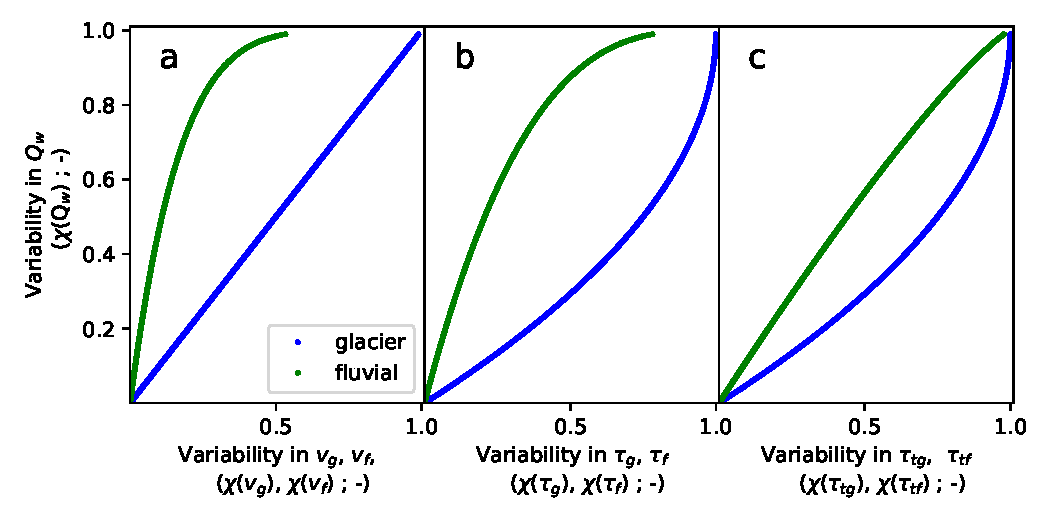
\includegraphics[width=0.8\linewidth]{multi_run_vars.pdf}
    \caption{Variability $\chi$ in velocity ($v_g$, $v_f$; a) shear stress ($\tau_g$, $\tau_f$; b) and width-integrated shear stress ($\tau_{tg}$, $\tau_{tf}$; c)  in glacial and subaerial systems. Values are determined from examining the same parameter space in Figure~\ref{fig:range}. }
    \label{fig:gammas}
  \end{figure}
\end{center}


\end{document}